\documentclass[a4paper,12pt,twoside]{memoir}

% Castellano
\usepackage[spanish,es-tabla]{babel}
\selectlanguage{spanish}
\usepackage[utf8]{inputenc}
\usepackage[T1]{fontenc}
\usepackage{lmodern} % scalable font
\usepackage{microtype}
\usepackage{placeins}

\RequirePackage{booktabs}
\RequirePackage[table]{xcolor}
\RequirePackage{xtab}
\RequirePackage{multirow}

% Links
\usepackage[colorlinks]{hyperref}
\hypersetup{
	allcolors = {red}
}

% Ecuaciones
\usepackage{amsmath}

% Rutas de fichero / paquete
\newcommand{\ruta}[1]{{\sffamily #1}}

% Párrafos
\nonzeroparskip


% Imagenes
\usepackage{graphicx}
\newcommand{\imagen}[2]{
	\begin{figure}[!h]
		\centering
		\includegraphics[width=0.9\textwidth]{#1}
		\caption{#2}\label{fig:#1}
	\end{figure}
	\FloatBarrier
}

\newcommand{\imagenflotante}[2]{
	\begin{figure}%[!h]
		\centering
		\includegraphics[width=0.9\textwidth]{#1}
		\caption{#2}\label{fig:#1}
	\end{figure}
}



% El comando \figura nos permite insertar figuras comodamente, y utilizando
% siempre el mismo formato. Los parametros son:
% 1 -> Porcentaje del ancho de página que ocupará la figura (de 0 a 1)
% 2 --> Fichero de la imagen
% 3 --> Texto a pie de imagen
% 4 --> Etiqueta (label) para referencias
% 5 --> Opciones que queramos pasarle al \includegraphics
% 6 --> Opciones de posicionamiento a pasarle a \begin{figure}
\newcommand{\figuraConPosicion}[6]{%
  \setlength{\anchoFloat}{#1\textwidth}%
  \addtolength{\anchoFloat}{-4\fboxsep}%
  \setlength{\anchoFigura}{\anchoFloat}%
  \begin{figure}[#6]
    \begin{center}%
      \Ovalbox{%
        \begin{minipage}{\anchoFloat}%
          \begin{center}%
            \includegraphics[width=\anchoFigura,#5]{#2}%
            \caption{#3}%
            \label{#4}%
          \end{center}%
        \end{minipage}
      }%
    \end{center}%
  \end{figure}%
}

%
% Comando para incluir imágenes en formato apaisado (sin marco).
\newcommand{\figuraApaisadaSinMarco}[5]{%
  \begin{figure}%
    \begin{center}%
    \includegraphics[angle=90,height=#1\textheight,#5]{#2}%
    \caption{#3}%
    \label{#4}%
    \end{center}%
  \end{figure}%
}
% Para las tablas
\newcommand{\otoprule}{\midrule [\heavyrulewidth]}
%
% Nuevo comando para tablas pequeñas (menos de una página).
\newcommand{\tablaSmall}[5]{%
 \begin{table}
  \begin{center}
   \rowcolors {2}{gray!35}{}
   \begin{tabular}{#2}
    \toprule
    #4
    \otoprule
    #5
    \bottomrule
   \end{tabular}
   \caption{#1}
   \label{tabla:#3}
  \end{center}
 \end{table}
}

%
%Para el float H de tablaSmallSinColores
\usepackage{float}

%
% Nuevo comando para tablas pequeñas (menos de una página).
\newcommand{\tablaSmallSinColores}[5]{%
 \begin{table}[H]
  \begin{center}
   \begin{tabular}{#2}
    \toprule
    #4
    \otoprule
    #5
    \bottomrule
   \end{tabular}
   \caption{#1}
   \label{tabla:#3}
  \end{center}
 \end{table}
}

\newcommand{\tablaApaisadaSmall}[5]{%
\begin{landscape}
  \begin{table}
   \begin{center}
    \rowcolors {2}{gray!35}{}
    \begin{tabular}{#2}
     \toprule
     #4
     \otoprule
     #5
     \bottomrule
    \end{tabular}
    \caption{#1}
    \label{tabla:#3}
   \end{center}
  \end{table}
\end{landscape}
}

%
% Nuevo comando para tablas grandes con cabecera y filas alternas coloreadas en gris.
\newcommand{\tabla}[6]{%
  \begin{center}
    \tablefirsthead{
      \toprule
      #5
      \otoprule
    }
    \tablehead{
      \multicolumn{#3}{l}{\small\sl continúa desde la página anterior}\\
      \toprule
      #5
      \otoprule
    }
    \tabletail{
      \hline
      \multicolumn{#3}{r}{\small\sl continúa en la página siguiente}\\
    }
    \tablelasttail{
      \hline
    }
    \bottomcaption{#1}
    \rowcolors {2}{gray!35}{}
    \begin{xtabular}{#2}
      #6
      \bottomrule
    \end{xtabular}
    \label{tabla:#4}
  \end{center}
}

%
% Nuevo comando para tablas grandes con cabecera.
\newcommand{\tablaSinColores}[6]{%
  \begin{center}
    \tablefirsthead{
      \toprule
      #5
      \otoprule
    }
    \tablehead{
      \multicolumn{#3}{l}{\small\sl continúa desde la página anterior}\\
      \toprule
      #5
      \otoprule
    }
    \tabletail{
      \hline
      \multicolumn{#3}{r}{\small\sl continúa en la página siguiente}\\
    }
    \tablelasttail{
      \hline
    }
    \bottomcaption{#1}
    \begin{xtabular}{#2}
      #6
      \bottomrule
    \end{xtabular}
    \label{tabla:#4}
  \end{center}
}

%
% Nuevo comando para tablas grandes sin cabecera.
\newcommand{\tablaSinCabecera}[5]{%
  \begin{center}
    \tablefirsthead{
      \toprule
    }
    \tablehead{
      \multicolumn{#3}{l}{\small\sl continúa desde la página anterior}\\
      \hline
    }
    \tabletail{
      \hline
      \multicolumn{#3}{r}{\small\sl continúa en la página siguiente}\\
    }
    \tablelasttail{
      \hline
    }
    \bottomcaption{#1}
  \begin{xtabular}{#2}
    #5
   \bottomrule
  \end{xtabular}
  \label{tabla:#4}
  \end{center}
}



\definecolor{cgoLight}{HTML}{EEEEEE}
\definecolor{cgoExtralight}{HTML}{FFFFFF}

%
% Nuevo comando para tablas grandes sin cabecera.
\newcommand{\tablaSinCabeceraConBandas}[5]{%
  \begin{center}
    \tablefirsthead{
      \toprule
    }
    \tablehead{
      \multicolumn{#3}{l}{\small\sl continúa desde la página anterior}\\
      \hline
    }
    \tabletail{
      \hline
      \multicolumn{#3}{r}{\small\sl continúa en la página siguiente}\\
    }
    \tablelasttail{
      \hline
    }
    \bottomcaption{#1}
    \rowcolors[]{1}{cgoExtralight}{cgoLight}

  \begin{xtabular}{#2}
    #5
   \bottomrule
  \end{xtabular}
  \label{tabla:#4}
  \end{center}
}




\graphicspath{ {./img/} }

% Capítulos
\chapterstyle{bianchi}
\newcommand{\capitulo}[2]{
	\setcounter{chapter}{#1}
	\setcounter{section}{0}
	\chapter*{#2}
	\addcontentsline{toc}{chapter}{#2}
	\markboth{#2}{#2}
}

% Apéndices
\renewcommand{\appendixname}{Apéndice}
\renewcommand*\cftappendixname{\appendixname}

\newcommand{\apendice}[1]{
	%\renewcommand{\thechapter}{A}
	\chapter{#1}
}

\renewcommand*\cftappendixname{\appendixname\ }

% Formato de portada
\makeatletter
\usepackage{xcolor}
\newcommand{\tutor}[1]{\def\@tutor{#1}}
\newcommand{\course}[1]{\def\@course{#1}}
\definecolor{cpardoBox}{HTML}{E6E6FF}
\def\maketitle{
  \null
  \thispagestyle{empty}
  % Cabecera ----------------
\noindent
\includegraphics[width=\textwidth]{cabecera}\vspace{1cm}%
  \vfill
  % Título proyecto y escudo informática ----------------
  \colorbox{cpardoBox}{%
    \begin{minipage}{.8\textwidth}
      \vspace{.5cm}\Large
      \begin{center}
      \textbf{TFG del Grado en Ingeniería Informática}\vspace{.6cm}\\
      \textbf{\LARGE\@title{}}
      \end{center}
      \vspace{.2cm}
    \end{minipage}

  }%
  \hfill\begin{minipage}{.20\textwidth}
    
\includegraphics[width=\textwidth]{escudoInfor}
  \end{minipage}
  \vfill
  % Datos de alumno, curso y tutores ------------------
  \begin{center}%
  {%
    \noindent\LARGE
    Presentado por \@author{}\\ 
    en Universidad de Burgos --- \@date{}\\
    Tutor: \@tutor{}\\
  }%
  \end{center}%
  \null
  \cleardoublepage
  }
\makeatother


% Datos de portada
\title{UBUSETAS 1.0 \\Documentación Técnica}
\author{Adrián Antón García}
\tutor{\\Dr. José F. Díez Pastor \\Dr. Raúl Marticorena Sánchez}
\date{\today}

\begin{document}

\maketitle



\cleardoublepage



%%%%%%%%%%%%%%%%%%%%%%%%%%%%%%%%%%%%%%%%%%%%%%%%%%%%%%%%%%%%%%%%%%%%%%%%%%%%%%%%%%%%%%%%



\frontmatter


\clearpage

% Indices
\tableofcontents

\clearpage

\listoffigures

\clearpage

\listoftables

\clearpage

\mainmatter

\appendix

\apendice{Plan de Proyecto Software}

\section{Introducción}

Sección en la que se va a desarrollar la planificación seguida en el proyecto, así como su viabilidad legal y económica.

Para llevar a cabo el seguimiento y planificación del proyecto se va a seguir la metodología \textit{Scrum} mediante Github, realizando un desarrollo incremental, dividido en sprints de una semana de duración cada uno. Durante cada sprint se irán creando y realizando las diferentes tareas correspondientes a los objetivos fijados en cada sprint. Al final de cada sprint se van a realizar las reuniones con los tutores para fijar las nuevas tareas de los nuevos sprints.

Para organizar las diferentes tareas se usará el tablero Kanban de Zenhub donde se mostrarán los diferentes estados de desarrollo en los que se encuentran las tareas.

El repositorio con el proyecto y las issues realizadas se puede encontrar en el siguiente enlace:
\url{https://github.com/AdrianAntonGarcia/-TFG-UBUSetas}

\section{Planificación temporal}

En esta sección se va a explicar la planificación del proyecto a través de los diferentes sprints realizados, explicando las fechas en las que se desarrollaron y que tareas se realizaron en cada uno. Los primeros cuatro sprint no se muestran de forma correcta debido a que no se cerraron las tareas de forma adecuada en esos sprint, este problema se arreglo a partir del quinto sprint.

Cada sprint estará acompañado de su grafo Burndown y un listado de las tareas realizadas. El proyecto se inicio el 11 de septiembre de 2017 y esta planeado entregarse en el 14 de enero de 2018, planificando así su desarrollo en cuatro meses.

\subsection{Sprint 1}

Este sprint se desarrollo entre los días 11 y 17 de septiembre de 2017. Se realizaron las siguientes tareas y objetivos:

\begin{itemize}
	\item Estudiar las propuestas de los tutores para elegir como desarrollar el clasificador.
	\item Empezar a estudiar las herramientas disponibles para entrenar los modelos.
	\item Elegir una propuesta para crear el clasificador.
\end{itemize}

La primera semana del proyecto se dedico a estudiar las diferentes técnicas propuestas para implementar el clasificador de imágenes, así como pensar las diferentes ventajas e inconvenientes de estas implementaciones y comprobar si eran viables con respecto al hardware y medios disponibles. Estas propuestas eran:
\begin{itemize}
	\item Crear un clasificador que se ejecute en un servidor y devuelva los resultados a la aplicación móvil. El modelo se puede reentrenar o entrenar desde cero.
	\item Reentrenar un modelo mediante la herramienta Tensorflow para poder ejecutar este modelo en el propio móvil.
\end{itemize}

\begin{figure}[h]
    \begin{center}%
        \begin{center}%
          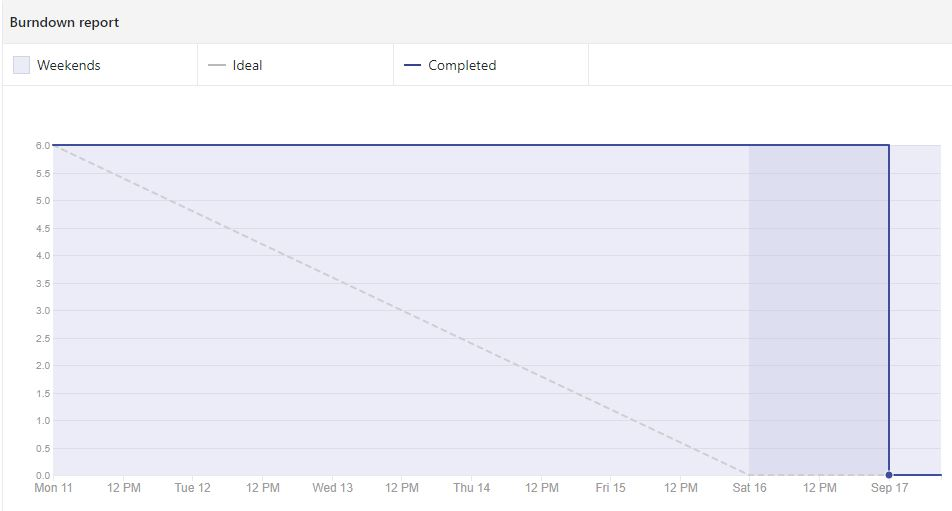
\includegraphics[width=1\textwidth]{imagenesAnexos/imagenesPlanificacion/sprint1}%
          \caption{Gráfico Burndown del sprint 1.}%
          \label{figSprint1}%
        \end{center}%
  	\end{center}%
\end{figure}%
\newpage

\subsection{Sprint 2}

Este sprint se desarrollo entre los días 18 y 24 de septiembre de 2017. Se realizaron las siguientes tareas y objetivos:

\begin{itemize}
	\item Estudiar las librerías de Tensorflow para el entrenamiento de los clasificadores.
	\item Estudiar los modelos Mobilenet e Inception.
	\item Estudiar como reentrenar los modelos mencionados.
	\item Estudiar como implementar los modelos en Android.
\end{itemize}

Esta semana relacionada con el segundo sprint se dedico principalmente al estudio de las diferentes técnicas disponibles para entrenar modelos que pudieran funcionar en una arquitectura móvil. Para ello se realizó el estudio de las librerías de Tensorflow y se siguieron los ejemplos para reentrenamiento disponibles en el repositorio de Github público de Tensorflow. 

Además se estudiaron las capacidades Hardware de las que disponíamos para entrenar estos modelos, ya que son procesos que requieren bastante tiempo de ejecucción y había que comprobar si podíamos reentrenar con los equipos disponibles.

\begin{figure}[h]
    \begin{center}%
        \begin{center}%
          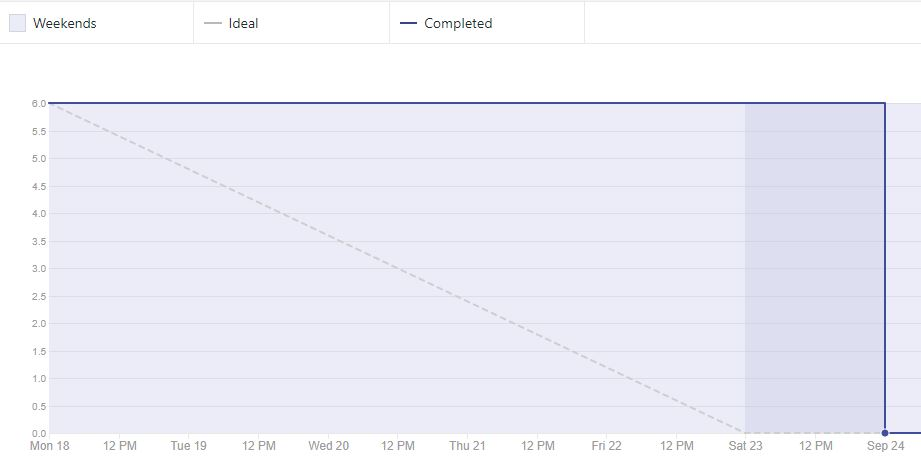
\includegraphics[width=1\textwidth]{imagenesAnexos/imagenesPlanificacion/sprint2}%
          \caption{Gráfico Burndown del sprint 2.}%
          \label{figSprint2}%
        \end{center}%
  	\end{center}%
\end{figure}%

\subsection{Sprint 3}

Este sprint se desarrollo entre el día 25 de septiembre y 1 de octubre de 2017. Se realizaron las siguientes tareas y objetivos:

\begin{itemize}
	\item Estudiar el entorno de programación Android Studio.
	\item Aprender a programar en Android.
	\item Implementar los modelos de clasificación en una aplicación Android.
\end{itemize}

El tercer sprint se dedico principalmente a familiarizarme a desarrollar en Android. El objetivo era el de tener una base para poder ir implementando los modelos Mobilenet e Inception en una aplicación de prueba Android.

Tras esta semana se consiguió una primera demo que ejecutaba un modelo Mobilenet en el propio dispositivo móvil, aunque no funcionaba correctamente y tenía errores que se corrigieron según se fue profundizando en los diferentes aspectos a estudiar.

\begin{figure}[h]
    \begin{center}%
        \begin{center}%
          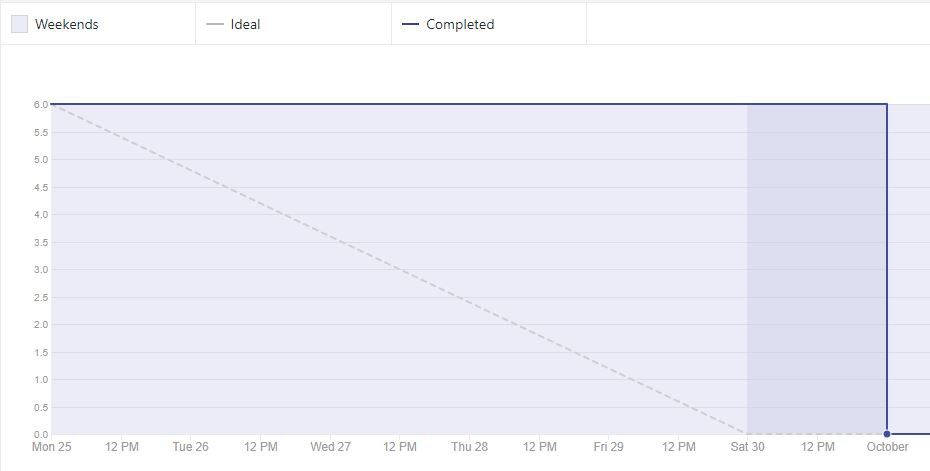
\includegraphics[width=1\textwidth]{imagenesAnexos/imagenesPlanificacion/sprint3}%
          \caption{Gráfico Burndown del sprint 3.}%
          \label{figSprint3}%
        \end{center}%
  	\end{center}%
\end{figure}%

\newpage

\subsection{Sprint 4}

Este sprint se desarrollo entre los días 2 y 8 de octubre de 2017. Se realizaron las siguientes tareas y objetivos:

\begin{itemize}
	\item Estudiar en que consistía y como realizar consultas a una web semántica.
	\item Estudiar el marco de definición de recursos \textit{RDF}.
	\item Estudiar el lenguaje de consultas \textit{SPARQL}, para realizar las consultas a una web semántica.
	\item Estudiar el funcionamiento de la \textit{DBpedia} como Web semántica.
	\item Estudio de la herramienta \textit{Apache Jena} para realizar estas consultas a través de un programa Java.
	
\end{itemize}

Esta semana tenía como objetivo el entender en que consistía una web semántica y como se podía implementar un programa Java que realizara consultas a una web semántica. El objetivo era el de estudiar como crear un programa Java que recopilara, de manera automática, información de las diferentes especies de setas.

Esta tarea tenía la complicación de que necesitábamos una web semántica que contuviera información de todas las setas, para poder facilitar la tarea de automatizar la extracción de información, y que esta se mostrará de manera uniforme. Tras estudiar las opciones disponibles se optó por la DBpedia ya que era la única que cumplía con las especificaciones necesarias y que contenía información suficiente de todas las especies.

\begin{figure}[h]
    \begin{center}%
        \begin{center}%
          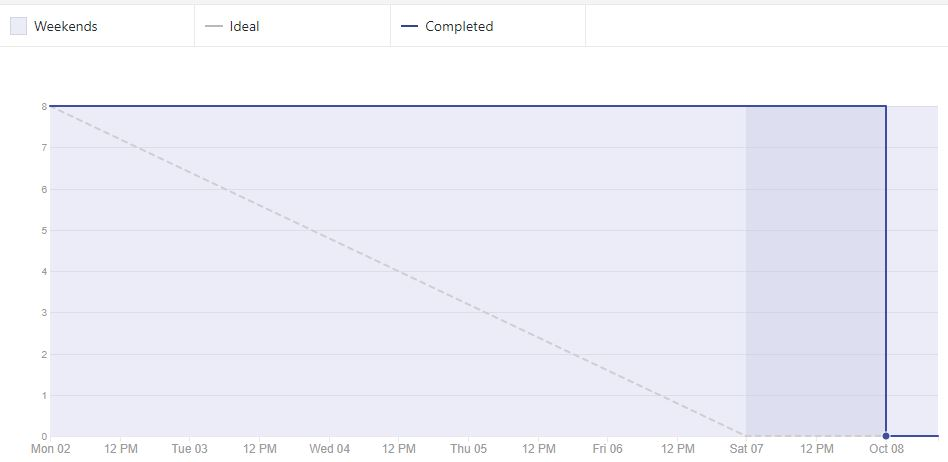
\includegraphics[width=1\textwidth]{imagenesAnexos/imagenesPlanificacion/sprint4}%
          \caption{Gráfico Burndown del sprint 4.}%
          \label{figSprint4}%
        \end{center}%
  	\end{center}%
\end{figure}%

Estos cuatro primeros sprints se dedicaron a estudiar las diferentes herramientas necesarias para implementar las propuestas del proyecto. La mayoría de estas herramientas eran desconocidas para mí por lo que me llevo un tiempo familiarizarme con ellas y empezar a implementar los diferentes programas.

En estos primeros sprints se consiguió crear en Android una aplicación que ejecutaba los modelos Mobilenet e Incpetion y en Java una aplicación que realizaba parte de las consultas necesarias a la DBpedia.

\subsection{Sprint 5}

Este sprint se desarrollo entre los días 11 y 18 de octubre de 2017. Se realizaron las siguientes tareas y objetivos:

\begin{itemize}
	\item Estudiar como implementar una base de datos SQL que funcione tanto en Android como en Windows.
	\item Implementar la base de datos en Windows para el programa de consultas a la web semántica.
	\item Implementar base de datos en la aplicación Android.
	\item Elegir una base de datos apropiada para los requisitos de la aplicación.
\end{itemize}

Para implementar la base de datos, se empezó estudiando e implementando una base de datos Microsoft JDBC en Windows con la intención de exportarla posteriormente a Android. Aunque se consiguió realizar esta parte, se decidió cambiar a una base de datos SQlite, ya que era mucho más ligera que la de Microsoft y más sencilla de usar para las necesidades básicas que tiene nuestra aplicación.

En esta semana se consiguió crear la base de datos y los métodos de acceso necesarios tanto en la aplicación Java como en la Android.

\begin{figure}[h]
    \begin{center}%
        \begin{center}%
          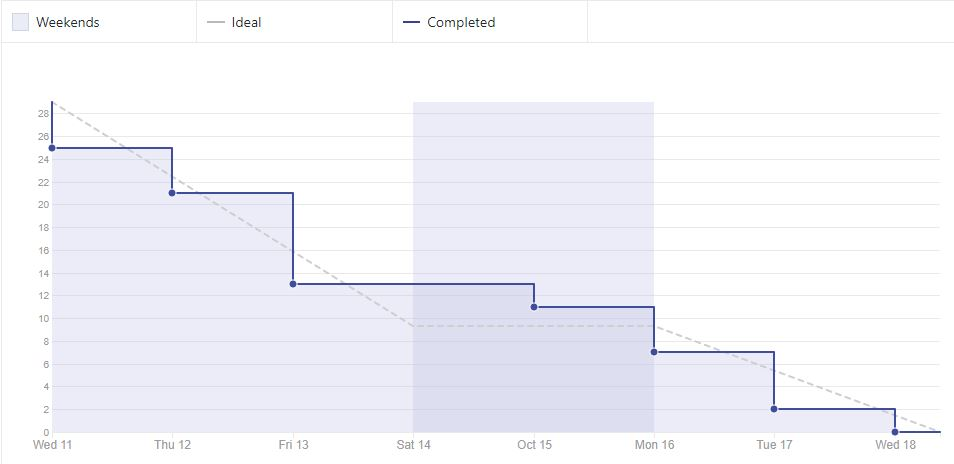
\includegraphics[width=0.9\textwidth]{imagenesAnexos/imagenesPlanificacion/sprint5}%
          \caption{Gráfico Burndown del sprint 5.}%
          \label{figSprint5}%
        \end{center}%
  	\end{center}%
\end{figure}%

\begin{figure}[h]
    \begin{center}%
        \begin{center}%
          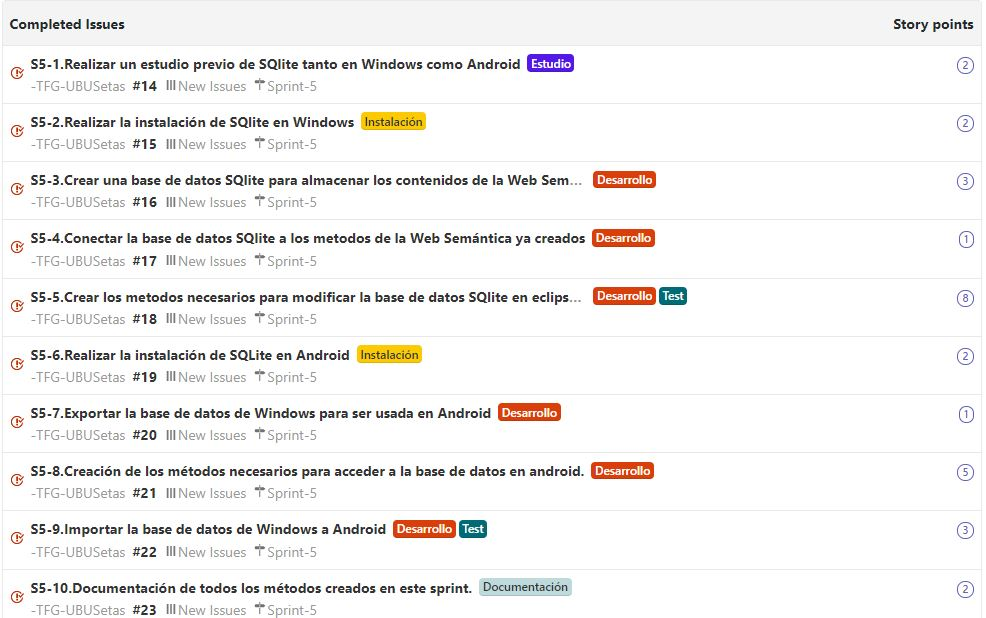
\includegraphics[width=0.9\textwidth]{imagenesAnexos/imagenesPlanificacion/tareas5}%
          \caption{Issues del sprint 5.}%
          \label{figTareas5}%
        \end{center}%
  	\end{center}%
\end{figure}%

\newpage

A partir de este sprint se empezó a utilizar de forma más correcta la Herramienta Zenhub y a mostrar de forma correcta las tareas desarrolladas en cada sprint.

\subsection{Sprint 6}

Este sprint se desarrollo entre los días 18 y 25 de octubre de 2017. Se realizaron las siguientes tareas y objetivos:

\begin{itemize}
	\item Crear la aplicación Java de acceso a la DBpedia a partir de las pruebas creadas.
	\item Crear la primera versión de la aplicación Android que muestre los resultados del clasificador.
	\item Crear un método en Java que traduzca textos de manera automática.
	\item Preparar la aplicación Android para mostrar los datos recibidos de la aplicación Java.
\end{itemize}

En esta semana se trabajo paralelamente tanto en la aplicación Android como en las consultas a la DBpedia. Se creo una versión Android que incorporaba las primeras actividades definidas en el prototipado. Se integro la información recogida por la aplicación Android en la base de datos de la aplicación Android.

Por último se creo un método Java que traducía realizando llamadas al traductor de Google, con el fin de entregar una aplicación internacionalizada tanto al español como el inglés.

\begin{figure}[h]
    \begin{center}%
        \begin{center}%
          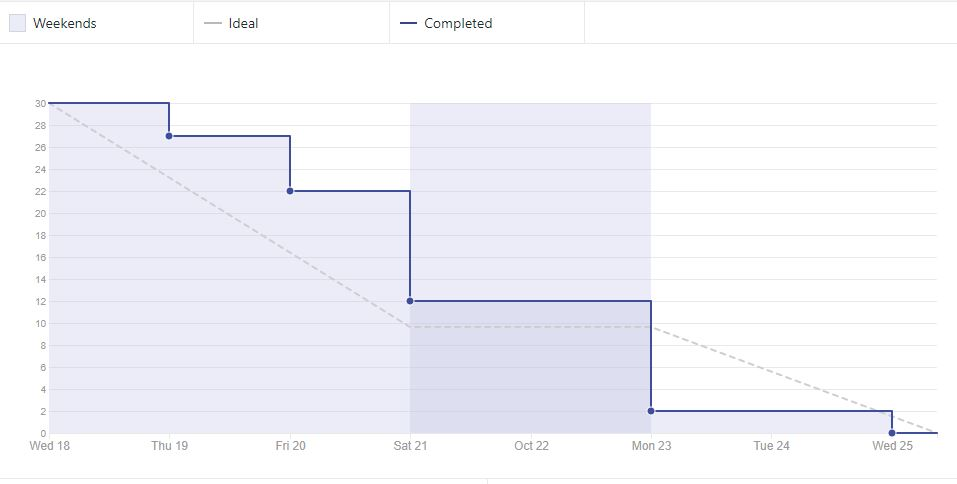
\includegraphics[width=0.9\textwidth]{imagenesAnexos/imagenesPlanificacion/sprint6}%
          \caption{Gráfico Burndown del sprint 6.}%
          \label{figSprint6}%
        \end{center}%
  	\end{center}%
\end{figure}%

\begin{figure}[h]
    \begin{center}%
        \begin{center}%
          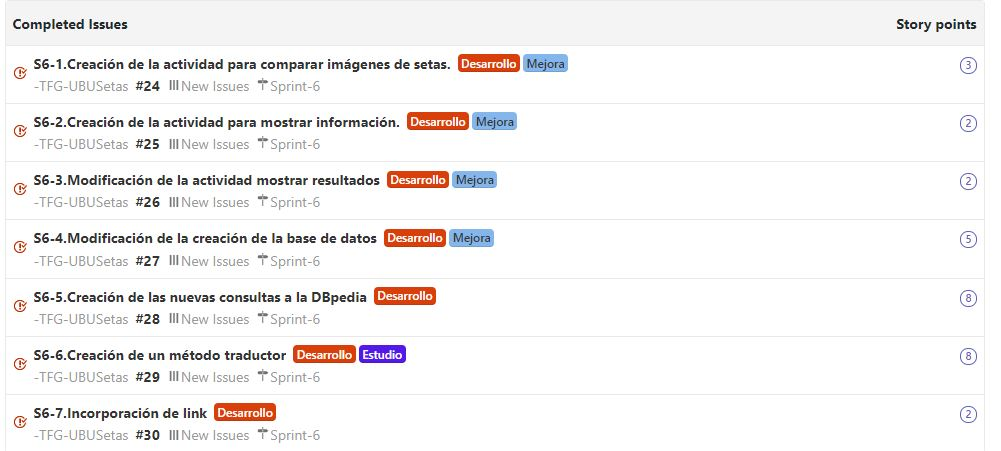
\includegraphics[width=0.9\textwidth]{imagenesAnexos/imagenesPlanificacion/tareas6}%
          \caption{Issues del sprint 6.}%
          \label{figTareas6}%
        \end{center}%
  	\end{center}%
\end{figure}%
\newpage

\subsection{Sprint 7}

Este sprint se desarrollo entre el día 25 de octubre y 1 de noviembre de 2017. Se realizaron las siguientes tareas y objetivos:

\begin{itemize}
	\item Estudiar como realizar Web Scraping en una página Web.
	\item Estudiar la herramienta \textit{Jaunt} para realizar Web Scraping en Java.
	\item Crear los métodos necesarios en el proyecto Java para extraer las claves dicotómicas de la página web \url{http://www.avelinosetas.info/claves.php}.
	\item Crear las actividades necesarias en la aplicación Android para mostrar las claves dicotómicas.
	\item Crear los métodos necesarios tanto en Android y Java para serializar las claves dicótomicas y transferirlas desde el proyecto Java a la aplicación Android.
\end{itemize}

En este sprint se encontró una página web con una clave dicotómica que contenía una gran cantidad de géneros de los clasificados por el clasificador, aunque no todos y mostraba claves de géneros para clasificar especies concretas de setas. Además la estructura html se repetía en todas las claves, lo que facilito la aplicación de las técnicas de Web Scraping.

Se decidió serializar las claves dicotómicas en estructuras de datos Java para exportar de manera sencilla las claves a la aplicación Android, sin necesidad de tener que usar las base de datos SQlite.

\begin{figure}[h]
    \begin{center}%
        \begin{center}%
          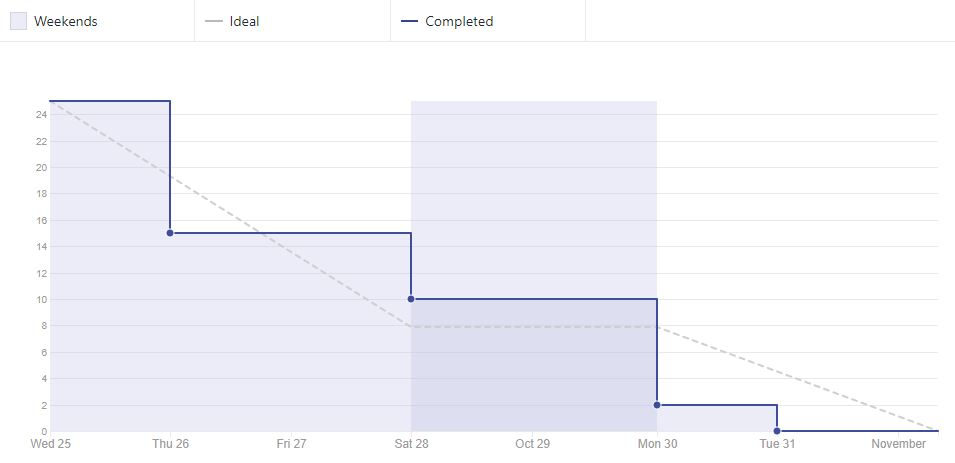
\includegraphics[width=0.9\textwidth]{imagenesAnexos/imagenesPlanificacion/sprint7}%
          \caption{Gráfico Burndown del sprint 7.}%
          \label{figSprint7}%
        \end{center}%
  	\end{center}%
\end{figure}%

\begin{figure}[h]
    \begin{center}%
        \begin{center}%
          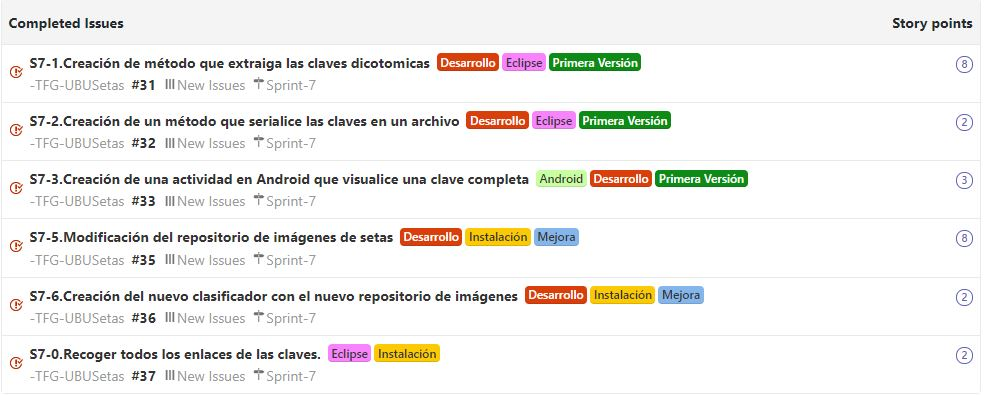
\includegraphics[width=0.9\textwidth]{imagenesAnexos/imagenesPlanificacion/tareas7}%
          \caption{Issues del sprint 7.}%
          \label{figTareas7}%
        \end{center}%
  	\end{center}%
\end{figure}%

\newpage

\subsection{Sprint 8}

Este sprint se desarrollo entre los días 2 y 8 de noviembre de 2017. Se realizaron las siguientes tareas y objetivos:

\begin{itemize}
	\item Extraer fotografías de las especies que se encuentran en la clave y no en el clasificador, con el fin de ampliar el número de especies recogidas por el clasificador.
	\item Reentrenar el clasificador con las nuevas imágenes recopiladas.
	\item Ajustar los métodos de la aplicación Java para que extraiga información de las nuevas especies.
	\item Añadir nueva información (género, comestibilidad y enlace)de las especies de setas para ser incorporada a la aplicación Android.
	\item Estudio de las directrices de \textit{material designs} para implementar la interfaz de la aplicación Android.
	\item Estudiar el funcionamiento de la herramienta Latex para empezar la memoria de la documentación.
\end{itemize}

En esta semana se decidió ampliar el número de especies clasificadas por el clasificador aumentando el número hasta las 171 especies. El objetivo era que no hubiera especies contenidas en la clave dicotómica de géneros que si estuvieran en el clasificador, con el fin de aprovechar la clave conseguida.

Esto provoco la modificación de los métodos en ambas aplicaciones para extraer y manejar las nuevas especies incorporadas.

También se empezó a estudiar como realizar una mejor interfaz basándome en los consejos ofrecidos por \textit{material designs}.

Se comenzó a estudiar la herramienta latex para empezar lo antes posible con la documentación del proyecto.

\begin{figure}[h]
    \begin{center}%
        \begin{center}%
          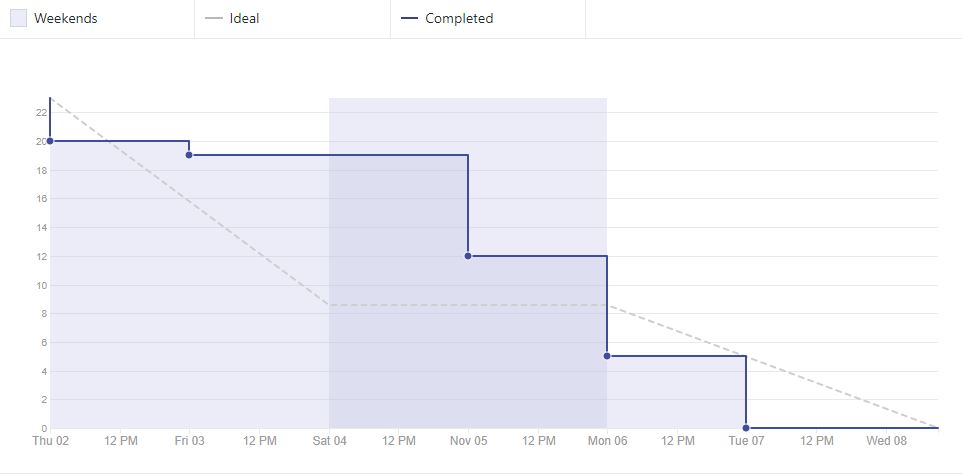
\includegraphics[width=0.9\textwidth]{imagenesAnexos/imagenesPlanificacion/sprint8}%
          \caption{Gráfico Burndown del sprint 8.}%
          \label{figSprint8}%
        \end{center}%
  	\end{center}%
\end{figure}%

\begin{figure}[h]
    \begin{center}%
        \begin{center}%
          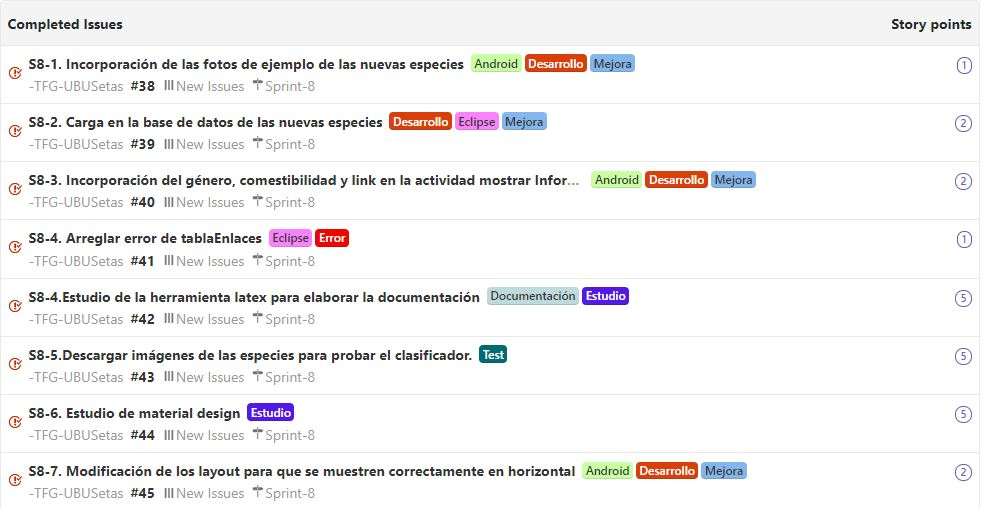
\includegraphics[width=0.9\textwidth]{imagenesAnexos/imagenesPlanificacion/tareas8}%
          \caption{Issues del sprint 8.}%
          \label{figTareas8}%
        \end{center}%
  	\end{center}%
\end{figure}%

\newpage

\subsection{Sprint 9}

Este sprint se desarrollo entre los días 8 y 15 de noviembre de 2017. Se realizaron las siguientes tareas y objetivos:

\begin{itemize}
	\item Escribir la introducción de la documentación.
	\item Escribir los objetivos del proyecto de la documentación.
	\item Escribir los conceptos teóricos de la documentación.
	\item Escribir las técnicas y herramientas de la documentación.
	\item Crear el prototipado para la interfaz de la aplicación Android.
\end{itemize}

Este sprint se dedicó a comenzar la documentación del proyecto y a crear un prototipado de la interfaz de la aplicación Android que sirviera de guía para construir la interfaz de la aplicación Android.

\begin{figure}[h]
    \begin{center}%
        \begin{center}%
          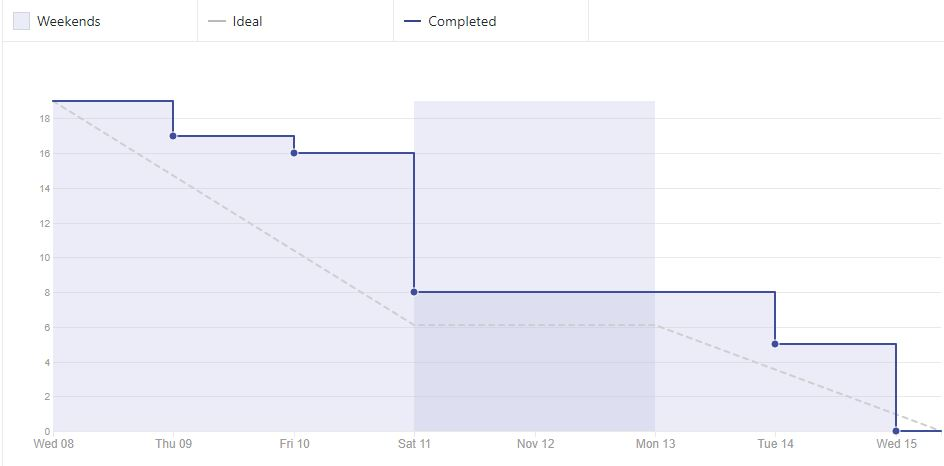
\includegraphics[width=0.9\textwidth]{imagenesAnexos/imagenesPlanificacion/sprint9}%
          \caption{Gráfico Burndown del sprint 9.}%
          \label{figSprint9}%
        \end{center}%
  	\end{center}%
\end{figure}%

\begin{figure}[h]
    \begin{center}%
        \begin{center}%
          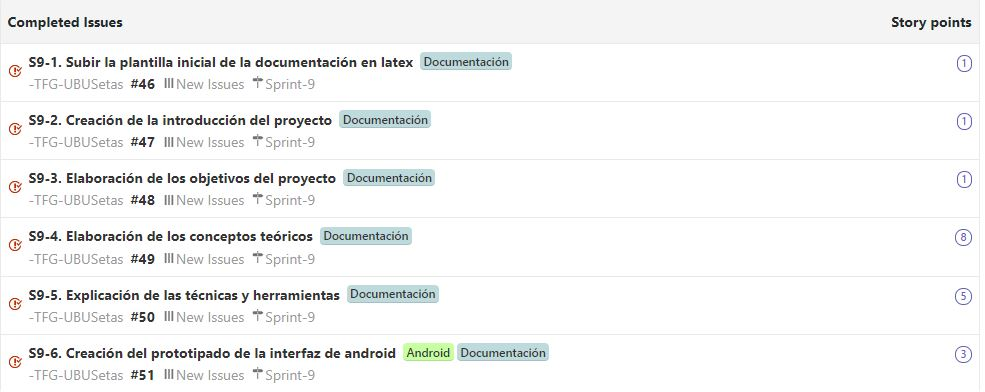
\includegraphics[width=0.9\textwidth]{imagenesAnexos/imagenesPlanificacion/tareas9}%
          \caption{Issues del sprint 9.}%
          \label{figTareas9}%
        \end{center}%
  	\end{center}%
\end{figure}%

\newpage

\subsection{Sprint 10}

Este sprint se desarrollo entre los días 15 y 22 de noviembre de 2017. Se realizaron las siguientes tareas y objetivos:

\begin{itemize}
	\item Construir la interfaz de las actividades creadas hasta este punto.
	\item Solucionar errores por los que las imágenes no se muestran correctamente en la aplicación Android.
	\item Seguir desarrollando la documentación.
	\item Creación de las actividades que muestran un listado de las especies y claves dicotómicas disponibles en la aplicación.
\end{itemize}

Esta semana se dedico a seguir construyendo la aplicación Android, incorporando dos nuevas actividades que mostraran al usuario las claves dicotómicas e información de las diferentes especies disponibles.

Se corrigió un error por el que el tamaño de la foto insertada por el usuario afectaba en los resultados ofrecidos por el clasificador, ya que se debían proporcionar imágenes escaladas a 224x224 pixeles de tamaño al clasificador para un correcto funcionamiento.

Se reviso la documentación creada en el sprint anterior.

\begin{figure}[h]
    \begin{center}%
        \begin{center}%
          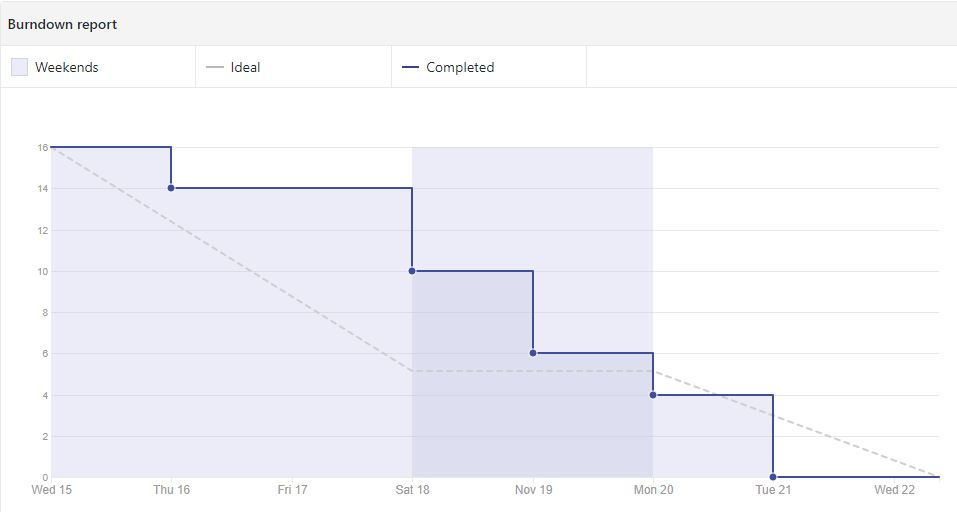
\includegraphics[width=0.9\textwidth]{imagenesAnexos/imagenesPlanificacion/sprint10}%
          \caption{Gráfico Burndown del sprint 10.}%
          \label{figSprint10}%
        \end{center}%
  	\end{center}%
\end{figure}%

\begin{figure}[h]
    \begin{center}%
        \begin{center}%
          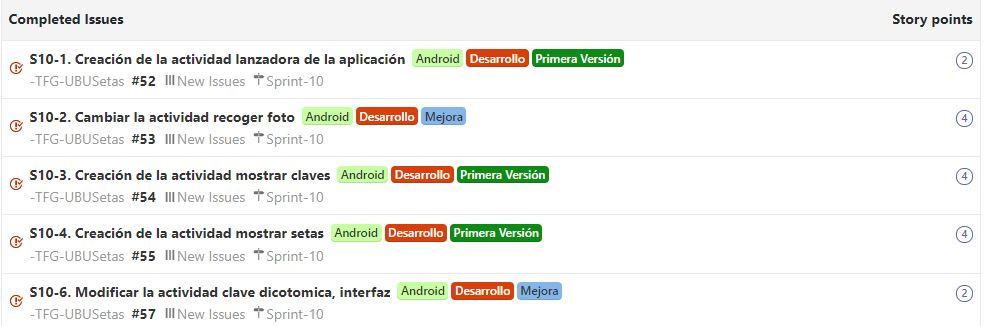
\includegraphics[width=0.9\textwidth]{imagenesAnexos/imagenesPlanificacion/tareas10}%
          \caption{Issues del sprint 10.}%
          \label{figTareas10}%
        \end{center}%
  	\end{center}%
\end{figure}%

\newpage

\subsection{Sprint 11}

Este sprint se desarrollo entre los días 22 y 30 de noviembre de 2017. Se realizaron las siguientes tareas y objetivos:

\begin{itemize}
	\item Seguir desarrollando la interfaz Android.
	\item Crear una actividad que pida al usuario elegir sobre que géneros, de los clasificados, desea aplicar la clave dicotómica para concretar las preguntas realizadas en esos géneros.
	\item Seguir desarrollando la documentación.
	\item Corregir pequeños errores de funcionamiento de la interfaz.
	\item Generar la primera release del proyecto.
\end{itemize}

En este sprint se siguió implementado la aplicación Android añadiendo nuevas funcionalidades, como el filtrado de géneros de la clave dicotómica. Así como corregir pequeños errores que se encontraron en la interfaz.

Tras realizar estas tareas se lanzo la primera release del proyecto.

Se terminaron los puntos de la memoria que no habían sido completados todavía.

\begin{figure}[h]
    \begin{center}%
        \begin{center}%
          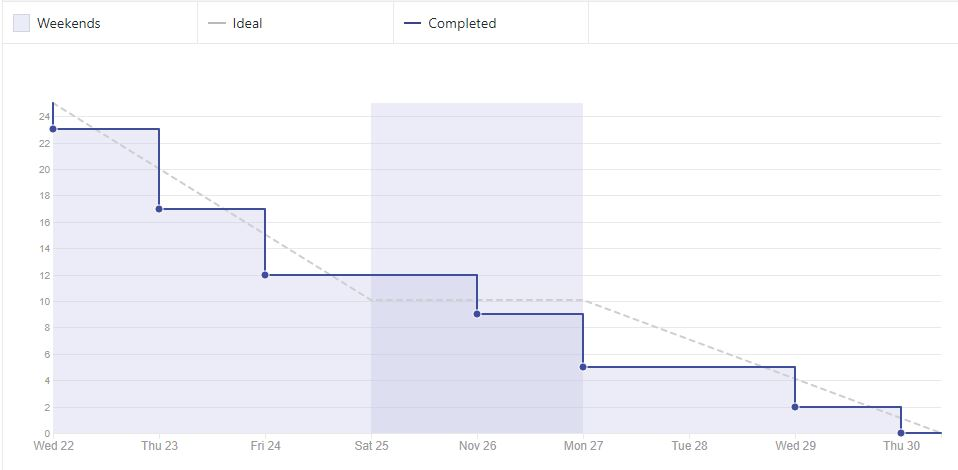
\includegraphics[width=0.9\textwidth]{imagenesAnexos/imagenesPlanificacion/sprint11}%
          \caption{Gráfico Burndown del sprint 11.}%
          \label{figSprint11}%
        \end{center}%
  	\end{center}%
\end{figure}%

\begin{figure}[h]
    \begin{center}%
        \begin{center}%
          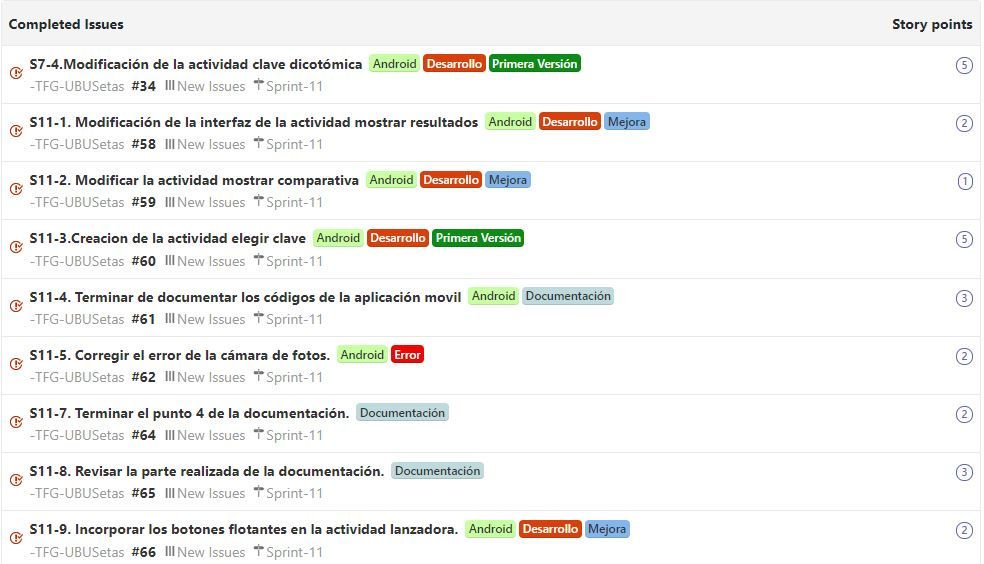
\includegraphics[width=0.9\textwidth]{imagenesAnexos/imagenesPlanificacion/tareas11}%
          \caption{Issues del sprint 11.}%
          \label{figTareas11}%
        \end{center}%
  	\end{center}%
\end{figure}%

\newpage

\subsection{Sprint 12}

Este sprint se desarrollo entre el día 30 de noviembre al 7 de diciembre de 2017. Se realizaron las siguientes tareas y objetivos:

\begin{itemize}
	\item Traducir todos los textos de la aplicación, claves e información al inglés.
	\item Internacionalizar la aplicación permitiendo que el usuario pueda elegir entre el español y el inglés, pudiendo cambiar en cualquier momento.
	\item Modificar el proyecto Java para que se traduzcan automáticamente todas las claves dicotómicas.
	\item Incorporar botones que muestren ayuda dentro de la aplicación al usuario en todas las actividades.
	\item Corregir errores en la rotación de pantalla de la aplicación Android.
\end{itemize}

Esta semana se dedico a traducir todos los textos de la aplicación Android al inglés, lo que provoco que se necesitara modificar el método extractor de claves dicotómicas del proyecto Java para que a la vez que extrajera las claves, las tradujera al inglés.

Se añadieron páginas de ayuda de usuario, dentro de la aplicación Android, para explicar la funcionalidad de cada elemento que se muestra al usuario en pantalla. Para acceder a ella, el usuario solo debe pulsar el botón de ayuda, o el item de ayuda disponible en el menú de la aplicación.

\begin{figure}[h]
    \begin{center}%
        \begin{center}%
          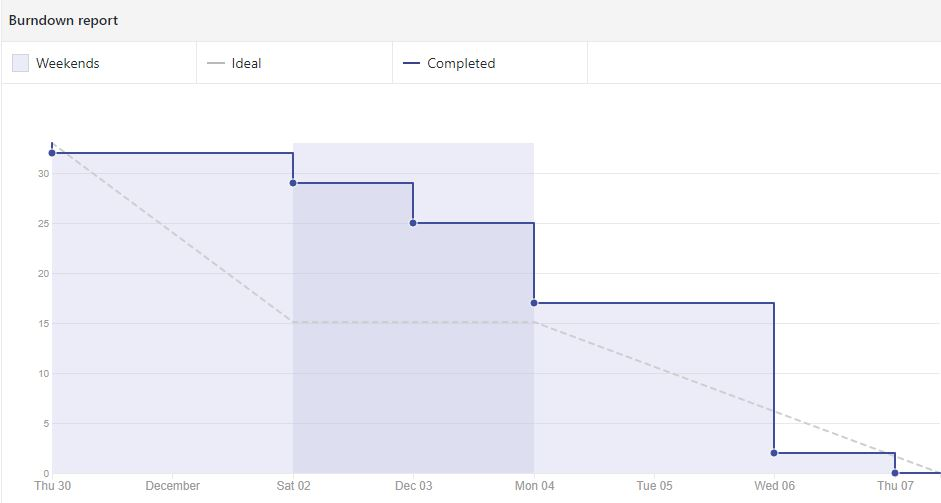
\includegraphics[width=0.9\textwidth]{imagenesAnexos/imagenesPlanificacion/sprint12}%
          \caption{Gráfico Burndown del sprint 12.}%
          \label{figSprint12}%
        \end{center}%
  	\end{center}%
\end{figure}%

\begin{figure}[h]
    \begin{center}%
        \begin{center}%
          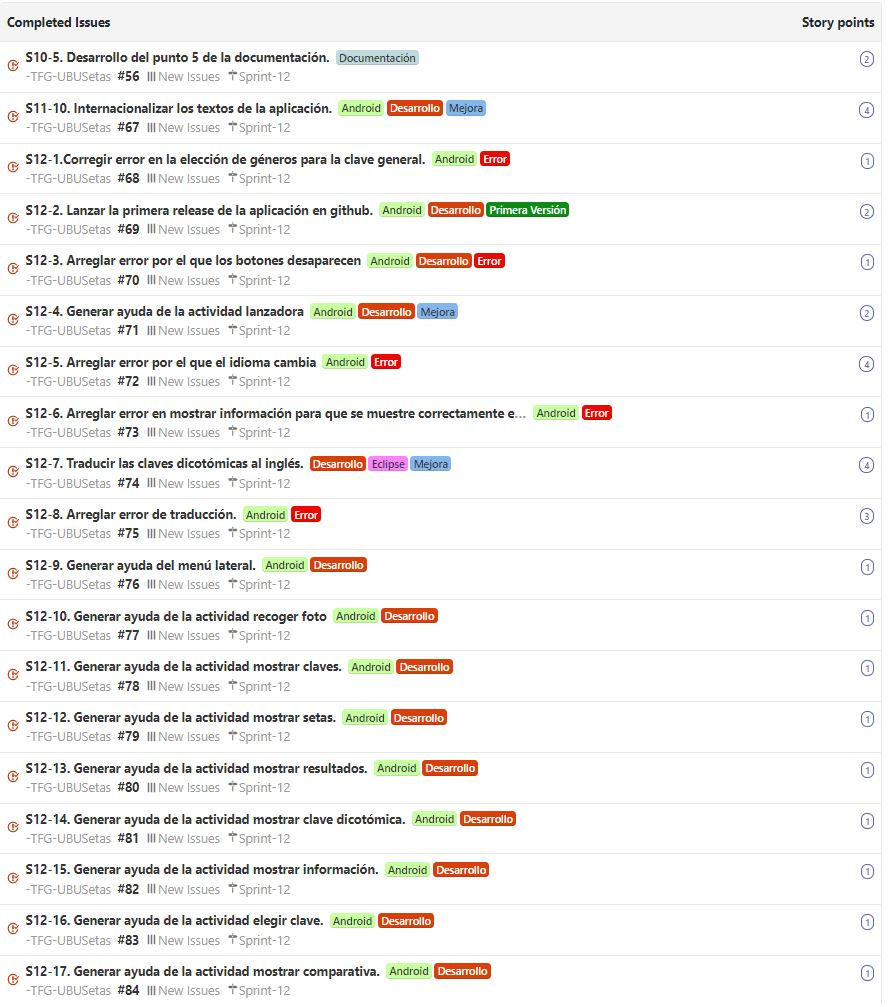
\includegraphics[width=0.9\textwidth]{imagenesAnexos/imagenesPlanificacion/tareas12}%
          \caption{Issues del sprint 12.}%
          \label{figTareas12}%
        \end{center}%
  	\end{center}%
\end{figure}%

\newpage

\subsection{Sprint 13}

Este sprint se desarrollo entre los días 7 y 14 de diciembre de 2017. Se realizaron las siguientes tareas y objetivos:

\begin{itemize}
	\item Estudiar la herramienta\textit{Roboelectric} para realizar los test unitarios en Android Studio.
	\item Estudiar las herramientas \textit{Espresso} y \textit{UIautomator} para realizar las pruebas de integración en Android Studio. 
	\item Realizar los primeros test unitarios de la aplicación.
	\item Incorporar botones que muestren ayuda dentro de la aplicación al usuario en todas las actividades.
	\item Escribir el punto de \textit{Aspectos relevantes del desarrollo
del proyecto} de la documentación.
	\item Escribir el punto de \textit{Trabajos relacioandos} de la documentación.
	\item Escribir el punto de \textit{Conclusiones y Líneas de trabajo
futuras} de la documentación.
\end{itemize}

Este sprint se dedico a estudiar como realizar los test unitarios y de integración a la aplicación Android.

Se elaborarón los primeros test unitarios y se siguió avanzando en el desarrollo de la documentación.

\begin{figure}[h]
    \begin{center}%
        \begin{center}%
          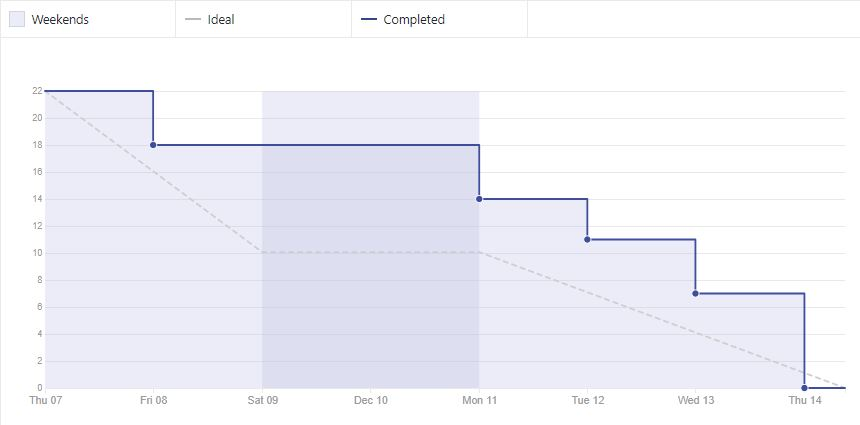
\includegraphics[width=0.9\textwidth]{imagenesAnexos/imagenesPlanificacion/sprint13}%
          \caption{Gráfico Burndown del sprint 13.}%
          \label{figSprint13}%
        \end{center}%
  	\end{center}%
\end{figure}%

\begin{figure}[h]
    \begin{center}%
        \begin{center}%
          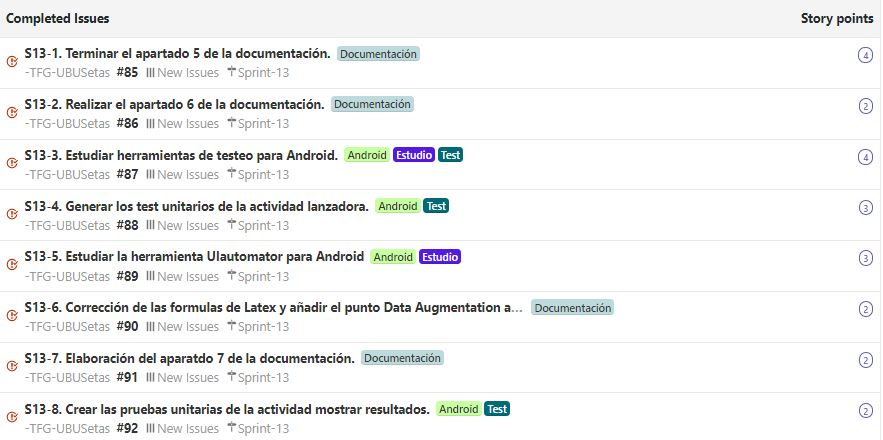
\includegraphics[width=0.9\textwidth]{imagenesAnexos/imagenesPlanificacion/tareas13}%
          \caption{Issues del sprint 13.}%
          \label{figTareas13}%
        \end{center}%
  	\end{center}%
\end{figure}%

\newpage

\subsection{Sprint 14}

Este sprint se desarrollo entre los días 14 y 21 de diciembre de 2017. Se realizaron las siguientes tareas y objetivos:

\begin{itemize}
	\item Realizar los test unitarios de todas las actividades de la aplicación Android.
	\item Realizar todos los test de integración de la aplicación Android.
	\item Estudiar la herramienta \textit{monkeyrunner} para crear test de rendimiento.
\end{itemize}

Este sprint se dedico a realizar pruebas unitarias y de intergación sobre todas las actividades de la aplicación Android.

También se estudio la herramienta monkeyrunner para crear una serie de eventos aleatorios sobre la aplicación y comprobar la robustez de esta.

\begin{figure}[h]
    \begin{center}%
        \begin{center}%
          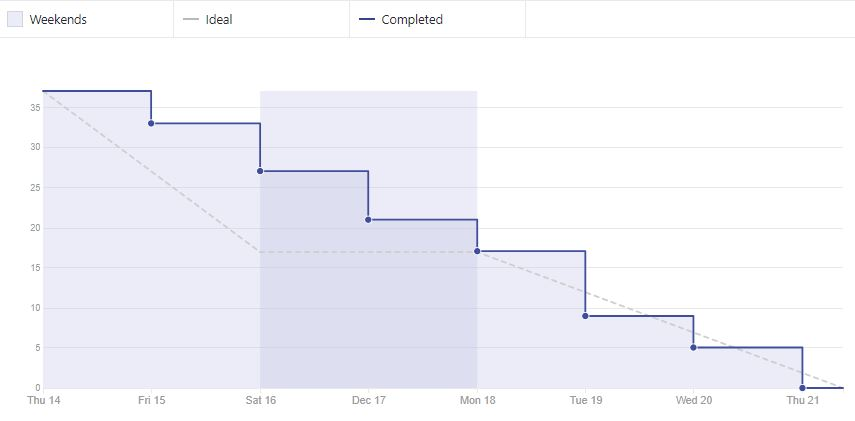
\includegraphics[width=0.9\textwidth]{imagenesAnexos/imagenesPlanificacion/sprint14}%
          \caption{Gráfico Burndown del sprint 14.}%
          \label{figSprint14}%
        \end{center}%
  	\end{center}%
\end{figure}%

\begin{figure}[h]
    \begin{center}%
        \begin{center}%
          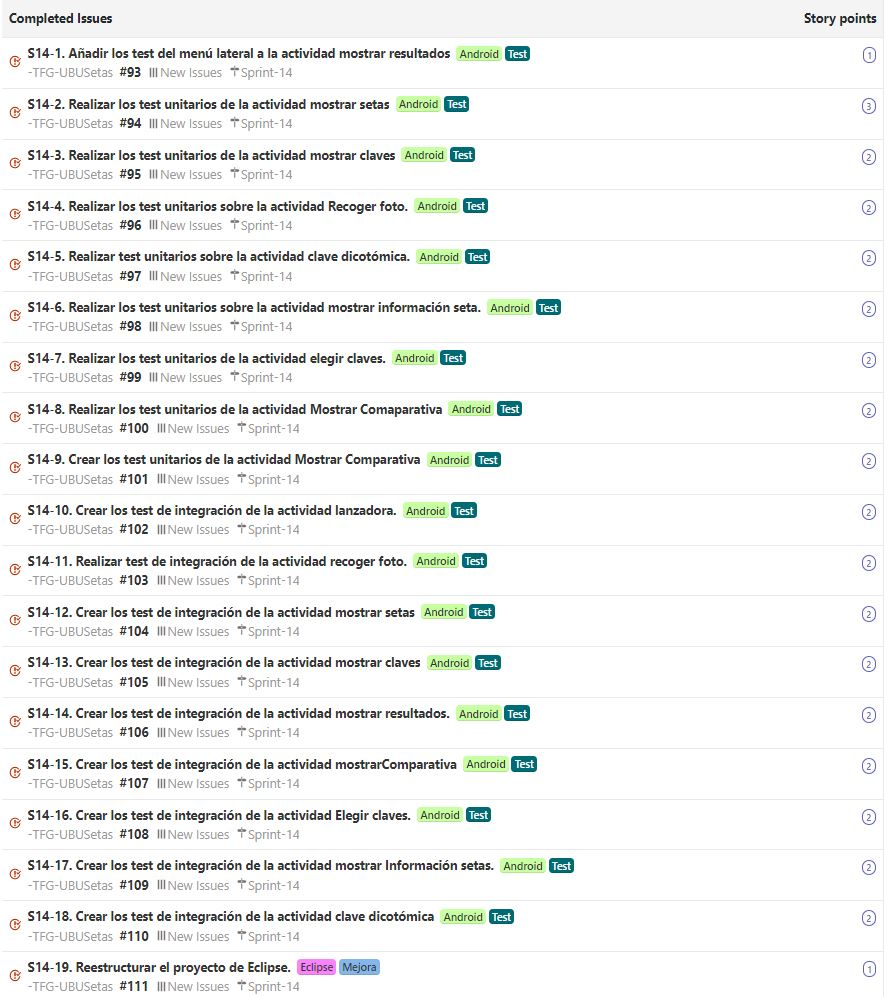
\includegraphics[width=0.9\textwidth]{imagenesAnexos/imagenesPlanificacion/tareas14}%
          \caption{Issues del sprint 14.}%
          \label{figTareas14}%
        \end{center}%
  	\end{center}%
\end{figure}%

\newpage
\newpage
\section{Estudio de viabilidad}
viabilidad
adads
ad
da
\subsection{Viabilidad económica}
asdsda
asds
\subsection{Viabilidad legal}
aada
adads
addd


\apendice{Especificación de Requisitos}

\section{Introducción}

En este apartado se van a detallar los requisitos globales del proyecto presentado, así como los diferentes casos de uso y requisitos funcionales implementados en la aplicación.

\section{Objetivos generales}

A continuación se muestran los objetivos generales del proyecto:

\begin{itemize}
	\item Investigar las bibliotecas de Tensorflow y los modelos Mobilenet e Inception para crear clasificadores de imágenes que sean capaces de ejecutarse en arquitecturas móviles.
	\item Investigar técnicas de uso de la Web Semántica para recopilar información de las diferentes especies de setas, de forma automática.
	\item Investigar técnicas de Web Scraping para extraer gran cantidad de información de una página Web.
	\item Implementar una aplicación Android que a partir de un clasificador de imágenes y la realización de preguntas al usuario, determine la especie de una seta. Esta aplicación mostrara información de cada especie y filtrará las preguntas de la clave dicotómica de acuerdo a las especies devueltas por el clasificador.
	\item Generar una aplicación Java que extraiga la información de las especies y las claves dicotómicas de forma automática.
	\item Internacionalizar la aplicación Android de manera que se pueda visualizar tanto en Inglés como en Español.
\end{itemize}

\section{Catalogo de requisitos}

En esta sección se van a detallar los diferentes requisitos funcionales implementados en las diferentes aplicaciones y herramientas.

\begin{itemize}
	\item \textbf{RF.1} Crear una herramienta que nos permita descargar información de las diferentes especies de setas.
	\begin{itemize}
	\item \textbf{RF.1.1} Se introducirá un listado de las especies deseadas y la aplicación devolverá la información extraída de la DBpedia.
	\item \textbf{RF.1.2} La información se podrá descargar tanto en 	español como en inglés.
	\end{itemize}
	
	\item \textbf{RF.2} Crear una herramienta que nos permita descargar las diferentes claves dicotómicas.
	\begin{itemize}
	\item \textbf{RF.2.1} La aplicación devolverá una clave dicotómica que discrimine entre géneros de setas.
	\item \textbf{RF.2.2} La aplicación devolverá claves dicotómicas que discriminen entre las especies de diferentes géneros de setas.
	\item \textbf{RF.2.3} Las claves se extraerán en español y se traducirán automáticamente al inglés.
	\item \textbf{RF.2.4} Las claves se serializarán en estructuras de datos java para incorporarlas a la aplicación Android.
	\end{itemize}
	
	\item \textbf{RF.3} Generar una aplicación para crear una base de datos SQlite para almacenar la información descargada y exportarla a la aplicación Android. Permitirá las siguientes acciones:
	\begin{itemize}
	\item \textbf{RF.3.1} Almacenar la descripción de la especie en Español.
	\item \textbf{RF.3.2} Almacenar la descripción de la especie en Inglés.
	\item \textbf{RF.3.3} Almacenar la comestibilidad de la especie en Español.
	\item \textbf{RF.3.4} Almacenar la comestibilidad de la especie en Inglés.
	\item \textbf{RF.3.5} Almacenar el género de la especie.
	\item \textbf{RF.3.6} Almacenar un enlace que redirija a la página web de la seta en Wikipedia.
	\end{itemize}
	
	\item \textbf{RF.4} Usar los algoritmos de Python proporcionados en los ejemplos de Tensorflow para entrenar los clasificadores de imágenes. \url{https://github.com/tensorflow/tensorflow/tree/master/tensorflow/examples/image_retraining}
	\begin{itemize}
	\item \textbf{RF.4.1} Elegir el modelo de Mobilenet o Inception.
	\item \textbf{RF.4.2} Incorporar las imágenes de las especies de setas sobre las que se quiere entrenar el clasificador.
	\item \textbf{RF.4.3} Determinar el porcentaje de imágenes que van a ser recortadas para crear nuevas.
	\item \textbf{RF.4.4} Determinar el porcentaje de imágenes que van a ser escaladas para crear nuevas.
	\item \textbf{RF.4.5} Determinar el porcentaje de imágenes que se va a rotar para crear nuevas.
	\item \textbf{RF.4.6} Determinar el porcentaje de imágenes sobre las que se va a modificar el brillo para crear nuevas.
	\item \textbf{RF.4.7} Elegir el número de pasos que va a realizar el clasificador para entrenar el modelo.
	\end{itemize}
	
	\item \textbf{RF.5} Generar una aplicación Android que permita la clasificación de la especie de una seta con las siguientes funcionaldades:
	\begin{itemize}
	\item \textbf{RF.5.1} El usuario podrá introducir una imagen de la seta desde la cámara del móvil para clasificar.
	\item \textbf{RF.5.2} El usuario podrá guardar la imagen capturada desde la cámara.
	\item \textbf{RF.5.3} El usuario podrá introducir una imagen de la seta desde la galería del móvil para clasificar.
	\item \textbf{RF.5.4} La aplicación mostrará las especies más probables clasificadas para la imagen introducida.
	\item \textbf{RF.5.5} Se mostrará información e imágenes de ejemplo para cada especie obtenida como resultado.
	\item \textbf{RF.5.6} El usuario podrá comparar su imagen con las proporcionadas por la aplicación 
	\item \textbf{RF.5.7} La aplicación realizará preguntas al usuario para clasificar la especie y reforzar la tarea de clasificación.
	\item \textbf{RF.5.8} Se podrán filtrar las preguntas realizadas para que solo se realicen sobre las especies deseadas.
	\item \textbf{RF.5.9} El usuario podrá cambiar el idioma de la aplicación entre español e inglés.
	\item \textbf{RF.5.10} El usuario podrá acceder a la información de todas las especies a través de un listado de estas.
	\item \textbf{RF.5.11} El usuario podrá acceder a las claves dicotómicas de las especies a través de un listado de estas.
	\item \textbf{RF.5.12} La aplicación mostrará páginas de ayuda que guíen al usuario dentro de la aplicación.
	
	\end{itemize}
	
\end{itemize}


\section{Especificación de requisitos}

\subsection{Diagramas de casos de uso}

\begin{figure}[]
    \begin{center}%
        \begin{center}%
          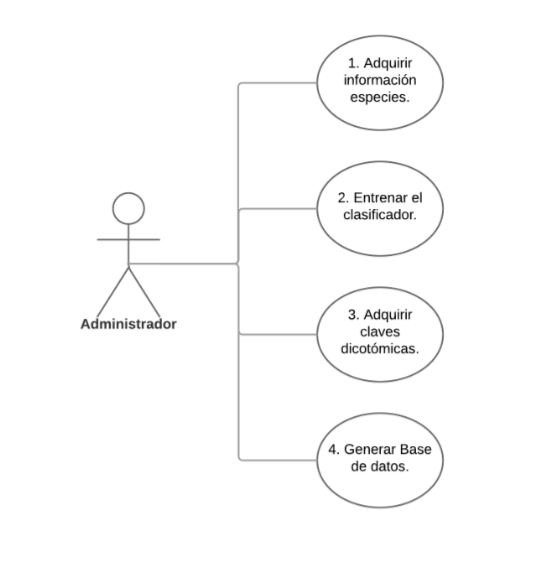
\includegraphics[width=1\textwidth]{imagenesAnexos/imagenesRequisitos/CasosDeUsoAdmin}%
          \caption{Diagrama de casos de uso del administrador.}%
          \label{figCasosUsoAdmin}%
        \end{center}%
  	\end{center}%
\end{figure}%

\begin{figure}[]
    \begin{center}%
        \begin{center}%
          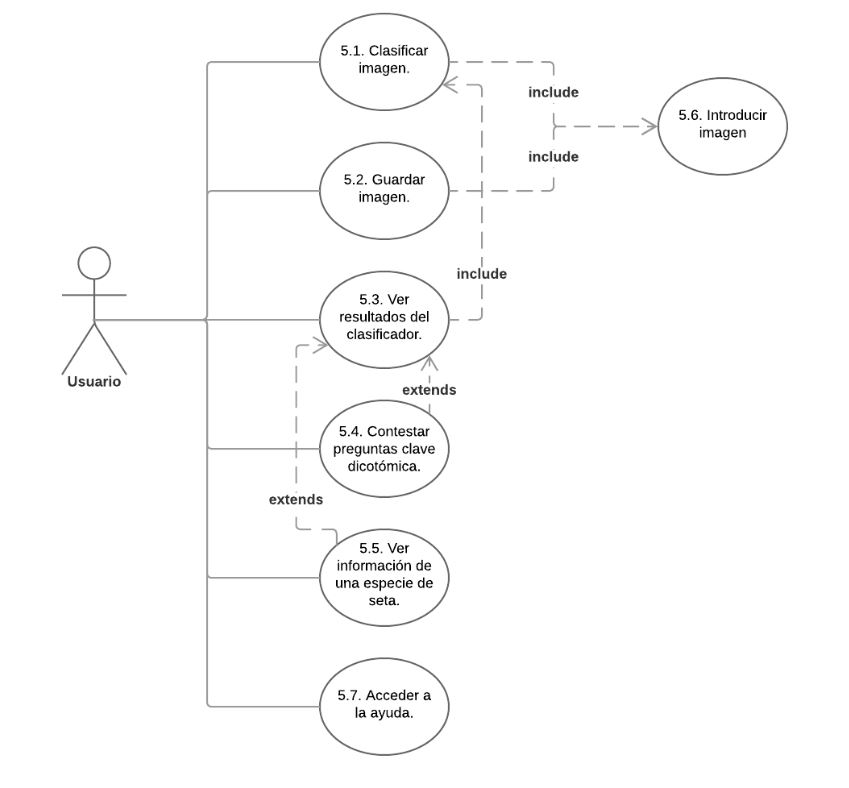
\includegraphics[width=1\textwidth]{imagenesAnexos/imagenesRequisitos/CasosDeUsoUser}%
          \caption{Diagrama de casos de uso del usuario.}%
          \label{figCasosUsoUser}%
        \end{center}%
  	\end{center}%
\end{figure}%
 
\newpage

\subsection{Especificación de los casos de uso}


%CASO DE USO 1

\tablaSmallSinColores{Caso de uso 1: Adquirir información especies.}{p{3cm} p{.75cm} p{9.5cm}}{tablaUC1}{
  \multicolumn{3}{l}{Caso de uso 1:  Adquirir información especies.} \\
 }
 {
  Descripción                            & \multicolumn{2}{p{10.25cm}}{Permite al administrador extraer la información de la especies de la DBpedia.} \\\hline
  \multirow{2}{3.5cm}{Requisitos}   &\multicolumn{2}{p{10.25cm}}{RF-1} \\\cline{2-3}
                                         & \multicolumn{2}{p{10.25cm}}{RF-1.1} \\\cline{2-3}
                                         & \multicolumn{2}{p{10.25cm}}{RF-1.2} 
                                         \\\hline
  Precondiciones                         &  \multicolumn{2}{p{10.25cm}}{Se necesita conexión a Internet para acceder a la DBpedia y tener creadas las tablas en la base de datos SQlite.}   \\\hline
  \multirow{2}{3.5cm}{Secuencia normal}  & Paso & Acción \\\cline{2-3}
                                         & 1    & El administrador indica la ruta de la base de datos.
  \\\cline{2-3}
                                         & 2    & Se inserta un listado de las especies a descargar.
  \\\cline{2-3}
                                         & 3    & Se inicia el programa
    \\\cline{2-3}
                                         & 4    & Se carga la base de datos con la información extraída de la DBpedia. 
                                         \\\hline
  Postcondiciones                        & \multicolumn{2}{p{10.25cm}}{Se ha descargado la información de la especies de setas.} \\\hline
  Excepciones                        & \multicolumn{2}{p{10.25cm}}{No se ha podido acceder a la DBpedia.}\\\hline
  Importancia                            & Media \\\hline
  Urgencia                               & Media \\
}

%CASO DE USO 2

\tablaSmallSinColores{Caso de uso 2: Entrenar el clasificador.}{p{3cm} p{.75cm} p{9.5cm}}{tablaUC2}{
  \multicolumn{3}{l}{Caso de uso 2: Entrenar el clasificador.} \\
 }
 {
  Descripción                            & \multicolumn{2}{p{10.25cm}}{Permite al administrador reentrenar el clasificador de imágenes.} \\\hline
  \multirow{2}{3.5cm}{Requisitos}   &\multicolumn{2}{p{10.25cm}}{RF-4} \\\cline{2-3}
                                         & \multicolumn{2}{p{10.25cm}}{RF-4.1} \\\cline{2-3}
                                         & \multicolumn{2}{p{10.25cm}}{RF-4.2} \\\cline{2-3}
                                         & \multicolumn{2}{p{10.25cm}}{RF-4.3} \\\cline{2-3}
                                         & \multicolumn{2}{p{10.25cm}}{RF-4.4} \\\cline{2-3}
                                         & \multicolumn{2}{p{10.25cm}}{RF-4.5} \\\cline{2-3}
                                         & \multicolumn{2}{p{10.25cm}}{RF-4.6} \\\cline{2-3}
                                         & \multicolumn{2}{p{10.25cm}}{RF-4.7}
                                         \\\hline
  Precondiciones                         &  \multicolumn{2}{p{10.25cm}}{Tener instalado Tensorflow y python en el sistema.}   \\\hline
  \multirow{2}{3.5cm}{Secuencia normal}  & Paso & Acción \\\cline{2-3}
                                         & 1    & Se indica el modelo a reentrenar.
  \\\cline{2-3}
                                         & 2    & Se incorporan las imágenes con las que se quiere entrenar.
  \\\cline{2-3}
                                         & 3    & Se ajustan los parámetros para realizar el Data Augmentation.
  \\\cline{2-3}
                                         & 4    & Se elige el número de pasos que va a realizar el programa para entrenar
  \\\cline{2-3}
                                         & 5    & Se inicia el programa.

                                         \\\hline
  Postcondiciones                        & \multicolumn{2}{p{10.25cm}}{Se ha entrenado un modelo para clasificar especies de setas.} \\\hline
  Excepciones                        & \multicolumn{2}{p{10.25cm}}{Número insuficiente de imágenes para entrenar.}\\\hline
  Importancia                            & Alta \\\hline
  Urgencia                               & Alta \\
}

%CASO DE USO 3

\tablaSmallSinColores{Caso de uso 3: Adquirir claves dicotómicas.}{p{3cm} p{.75cm} p{9.5cm}}{tablaUC3}{
  \multicolumn{3}{l}{Caso de uso 3: Adquirir claves dicotómicas.} \\
 }
 {
  Descripción                            & \multicolumn{2}{p{10.25cm}}{Permite al administrador extraer las claves de la página Web \url{http://www.avelinosetas.info/claves.php}.} \\\hline
  \multirow{2}{3.5cm}{Requisitos}   &\multicolumn{2}{p{10.25cm}}{RF-2} \\\cline{2-3}
                                         & \multicolumn{2}{p{10.25cm}}{RF-2.1} \\\cline{2-3}
                                         & \multicolumn{2}{p{10.25cm}}{RF-2.2} \\\cline{2-3}
                                         & \multicolumn{2}{p{10.25cm}}{RF-2.3} \\\cline{2-3}
                                         & \multicolumn{2}{p{10.25cm}}{RF-2.4} 
                                         \\\hline
  Precondiciones                         &  \multicolumn{2}{p{10.25cm}}{Se necesita conexión a Internet para acceder a la página web.}   \\\hline
  \multirow{2}{3.5cm}{Secuencia normal}  & Paso & Acción \\\cline{2-3}
                                         & 1    & El administrador indica el nombre del archivo donde se quiere exportar las claves.
  \\\cline{2-3}
                                         & 2    & Se inserta un listado de las claves a descargar.
  \\\cline{2-3}
                                         & 3    & Se inicia el programa
    \\\cline{2-3}
                                         & 4    & Se descargan las claves y se serializan en el archivo indicado.
                                         \\\hline
  Postcondiciones                        & \multicolumn{2}{p{10.25cm}}{Se obtienen las claves en un archivo serializado para ser exportado a la aplicación Android.} \\\hline
  Excepciones                        & \multicolumn{2}{p{10.25cm}}{No se ha podido acceder a la página web.}\\\hline
  Importancia                            & Alta \\\hline
  Urgencia                               & Media \\
}

%CASO DE USO 4

\tablaSmallSinColores{Caso de uso 4: Generar Base de datos.}{p{3cm} p{.75cm} p{9.5cm}}{tablaUC4}{
  \multicolumn{3}{l}{Caso de uso 4: Generar Base de datos.} \\
 }
 {
  Descripción                            & \multicolumn{2}{p{10.25cm}}{Permite al administrador preparar la base de datos para almacenar la información de las setas.} \\\hline
  \multirow{2}{3.5cm}{Requisitos}   &\multicolumn{2}{p{10.25cm}}{RF-1} \\\cline{2-3}
                                         & \multicolumn{2}{p{10.25cm}}{RF-2}
                                         \\\hline
  Precondiciones                         &  \multicolumn{2}{p{10.25cm}}{Haber creado una base de datos SQlite en el sistema.}   \\\hline
  \multirow{2}{3.5cm}{Secuencia normal}  & Paso & Acción \\\cline{2-3}
                                         & 1    & El administrador indica la ruta donde se encuentra la base de datos SQlite.
  \\\cline{2-3}
                                         & 2    & Se inicia el programa.
  \\\cline{2-3}
                                         & 3    & El programa crea las tablas necesarias en la base de datos.
                                         \\\hline
  Postcondiciones                        & \multicolumn{2}{p{10.25cm}}{Se crean las tablas en la base de datos.} \\\hline
  Excepciones                        & \multicolumn{2}{p{10.25cm}}{Excepción SQL.}\\\hline
  Importancia                            & Media \\\hline
  Urgencia                               & Media \\
}

%CASO DE USO 5

\tablaSmallSinColores{Caso de uso 5.1: Clasificar imagen.}{p{3cm} p{.75cm} p{9.5cm}}{tablaUC5}{
  \multicolumn{3}{l}{Caso de uso 5.1: Clasificar imagen.} \\
 }
 {
  Descripción                            & \multicolumn{2}{p{10.25cm}}{Permite al usuario clasificar la especie a la que pertenece la seta que aparezca en la foto introducida.} \\\hline
  \multirow{2}{3.5cm}{Requisitos}   &\multicolumn{2}{p{10.25cm}}{RF-5} \\\cline{2-3}
                                         & \multicolumn{2}{p{10.25cm}}{RF-5.4}
                                         \\\hline
  Precondiciones                         &  \multicolumn{2}{p{10.25cm}}{Haber cargado la imagen a clasificar.}   \\\hline
  \multirow{2}{3.5cm}{Secuencia normal}  & Paso & Acción \\\cline{2-3}
                                         & 1    & El usuario pulsa en el botón de clasificar, bien desde la actividad lanzadora o desde el menú.
  \\\cline{2-3}
                                         & 2    & El usuario carga la imagen deseada.
  \\\cline{2-3}
                                         & 3    & El usuario pulsa sobre el botón de clasificar la imagen.
  \\\cline{2-3}
                                         & 4    & El sistema muestra las especies más probables clasificadas para esa imagen.
                                         \\\hline
  Postcondiciones                        & \multicolumn{2}{p{10.25cm}}{Se muestran los resultados obtenidos.} \\\hline
  Excepciones                        & \multicolumn{2}{p{10.25cm}}{Error en la carga de la imágen. Error en la clasificación.}\\\hline
  Importancia                            & Alta \\\hline
  Urgencia                               & Alta \\
}

%CASO DE USO 6

\tablaSmallSinColores{Caso de uso 5.2: Guardar imagen.}{p{3cm} p{.75cm} p{9.5cm}}{tablaUC6}{
  \multicolumn{3}{l}{Caso de uso 5.2: Guardar imagen.} \\
 }
 {
  Descripción                            & \multicolumn{2}{p{10.25cm}}{Permite al usuario guardar en el sistema la imagen que haya capturado desde el móvil.} \\\hline
  \multirow{2}{3.5cm}{Requisitos}   &\multicolumn{2}{p{10.25cm}}{RF-5} \\\cline{2-3}
                                         & \multicolumn{2}{p{10.25cm}}{RF-5.2}
                                         \\\hline
  Precondiciones                         &  \multicolumn{2}{p{10.25cm}}{Tener acceso a la cámara del móvil.}   \\\hline
  \multirow{2}{3.5cm}{Secuencia normal}  & Paso & Acción \\\cline{2-3}
                                         & 1    & El usuario pulsa en el botón de clasificar, bien desde la actividad lanzadora o desde el menú.
  \\\cline{2-3}
                                         & 2    & El usuario elije la opción de cargar la imagen desde el móvil.
  \\\cline{2-3}
                                         & 3    & Se introduce la imagen.
  \\\cline{2-3}
                                         & 4    & El usuario pulsa sobre el botón de guardar.
                                         \\\hline
  Postcondiciones                        & \multicolumn{2}{p{10.25cm}}{Se almacena la imagen en la galería del móvil.} \\\hline
  Excepciones                        & \multicolumn{2}{p{10.25cm}}{Error en la carga de la imágen. Error al adquirir los permisos del móvil.}\\\hline
  Importancia                            & Baja \\\hline
  Urgencia                               & Baja \\
}

%CASO DE USO 7

\tablaSmallSinColores{Caso de uso 5.3: Ver resultados del clasificador.}{p{3cm} p{.75cm} p{9.5cm}}{tablaUC7}{
  \multicolumn{3}{l}{Caso de uso 5.3: Ver resultados del clasificador.} \\
 }
 {
  Descripción                            & \multicolumn{2}{p{10.25cm}}{Permite al usuario ver los resultados obtenidos de la clasificación y obtener información de las especies.} \\\hline
  \multirow{2}{3.5cm}{Requisitos}   &\multicolumn{2}{p{10.25cm}}{RF-5} \\\cline{2-3}
                                         & \multicolumn{2}{p{10.25cm}}{RF-5.4}
                                         \\\cline{2-3}
                                         & \multicolumn{2}{p{10.25cm}}{RF-5.5}
                                         \\\cline{2-3}
                                         & \multicolumn{2}{p{10.25cm}}{RF-5.6}
                                         \\\hline
  Precondiciones                         &  \multicolumn{2}{p{10.25cm}}{}   \\\hline
  \multirow{2}{3.5cm}{Secuencia normal}  & Paso & Acción \\\cline{2-3}
                                         & 1    & El usuario ha clasificado una imagen.
  \\\cline{2-3}
                                         & 2    & El sistema muestra una lista con los resultados obtenidos.
  \\\cline{2-3}
                                         & 3    & Si el usuario pulsa una especie de los resultados, se mostrará una imagen de ejemplo que se comparará con la introducida por el usuario.
  \\\cline{2-3}
                                         & 4    & Si el usuario mantiene pulsada una especie de los resultados, se mostrará información describiendo la especie.
                                         \\\hline
  Postcondiciones                        & \multicolumn{2}{p{10.25cm}}{Se muestra información de los resultados} \\\hline
  Excepciones                        & \multicolumn{2}{p{10.25cm}}{Error en la carga de la imágen. Error al acceder a la base de datos.}\\\hline
  Importancia                            & Media \\\hline
  Urgencia                               & Media \\
}

%CASO DE USO 8

\tablaSmallSinColores{Caso de uso 5.4: Contestar preguntas clave dicotómica.}{p{3cm} p{.75cm} p{9.5cm}}{tablaUC8}{
  \multicolumn{3}{l}{Caso de uso 5.4: Contestar preguntas clave dicotómica.} \\
 }
 {
  Descripción                            & \multicolumn{2}{p{10.25cm}}{El sistema realiza una serie de preguntas al usuario con el fin de clasificar el género o especie de la seta.} \\\hline
  \multirow{2}{3.5cm}{Requisitos}   &\multicolumn{2}{p{10.25cm}}{RF-5} \\\cline{2-3}
                                         & \multicolumn{2}{p{10.25cm}}{RF-5.7}
                                         \\\cline{2-3}
                                         & \multicolumn{2}{p{10.25cm}}{RF-5.8}
                                         \\\hline
  Precondiciones                         &  \multicolumn{2}{p{10.25cm}}{}   \\\hline
  \multirow{2}{3.5cm}{Secuencia después de clasificar una imagen.}  & Paso & Acción \\\cline{2-3}
                                         & 1    & El usuario clasifica una imagen.
  \\\cline{2-3}
                                         & 2    & Se pulsa el botón de acceder a la clave dicotómica.
  \\\cline{2-3}
                                         & 3    & El usuario puede elegir sobre que especies filtrar las preguntas o realizar todas las preguntas.
  \\\cline{2-3}
                                         & 4    & Una vez seleccionadas las especies, se pulsa sobre el botón de clasificar.
  \\\cline{2-3}
                                         & 5    & El usuario va respondiendo a las preguntas que le aparecen hasta que se muestra la especie clasificada.
                                         \\\hline
                                         \multirow{2}{3.5cm}{Secuencia desde el listado de claves}  & Paso & Acción \\\cline{2-3}
                                         & 1    & El usuario pulsa el botón de mostrar claves.
  \\\cline{2-3}
                                         & 2    & El sistema muestra una lista con las claves disponibles.
  \\\cline{2-3}
                                         & 3    & El usuario elije una clave.
  \\\cline{2-3}
                                         & 4    & El usuario va respondiendo a las preguntas que le aparecen hasta que se muestra la especie clasificada.
                                         \\\hline
  Postcondiciones                        & \multicolumn{2}{p{10.25cm}}{Se clasifica la especie de la seta mediante una clave dicotómica.} \\\hline
  Excepciones                        & \multicolumn{2}{p{10.25cm}}{}\\\hline
  Importancia                            & Alta \\\hline
  Urgencia                               & Alta \\
}

%CASO DE USO 9

\tablaSmallSinColores{Caso de uso 5.5: Ver información de una especie de seta.}{p{3cm} p{.75cm} p{9.5cm}}{tablaUC9}{
  \multicolumn{3}{l}{Caso de uso 5.5: Ver información de una especie de seta.} \\
 }
 {
  Descripción                            & \multicolumn{2}{p{10.25cm}}{El sistema muestra información de una especie de seta.} \\\hline
  \multirow{2}{3.5cm}{Requisitos}   &\multicolumn{2}{p{10.25cm}}{RF-5} \\\cline{2-3}
                                         & \multicolumn{2}{p{10.25cm}}{RF-5.10}
                                         \\\cline{2-3}
                                         & \multicolumn{2}{p{10.25cm}}{RF-5.5}
                                         \\\hline
  Precondiciones                         &  \multicolumn{2}{p{10.25cm}}{}   \\\hline
  \multirow{2}{3.5cm}{Secuencia desde los resultados.}  & Paso & Acción \\\cline{2-3}
                                         & 1    & El usuario clasifica una imagen.
  \\\cline{2-3}
                                         & 2    & Se mantiene pulsado sobre uno de los resultados.
  \\\cline{2-3}
                                         & 3    & El sistema muestra información de la especie seleccionada.
                                         \\\hline
                                         \multirow{2}{3.5cm}{Secuencia desde el listado de especies.}  & Paso & Acción \\\cline{2-3}
                                         & 1    & El usuario pulsa el botón de mostrar setas.
  \\\cline{2-3}
                                         & 2    & El sistema muestra una lista con las especies de setas disponibles.
  \\\cline{2-3}
                                         & 3    & El usuario elije una especie.
  \\\cline{2-3}
                                         & 4    & El sistema muestra información de la especie seleccionada.
                                         \\\hline
  Postcondiciones                        & \multicolumn{2}{p{10.25cm}}{Se muestra información de la especie seleccionada.} \\\hline
  Excepciones                        & \multicolumn{2}{p{10.25cm}}{}\\\hline
  Importancia                            & Media \\\hline
  Urgencia                               & Media \\
}

%CASO DE USO 10

\tablaSmallSinColores{Caso de uso 5.6: Introducir imagen.}{p{3cm} p{.75cm} p{9.5cm}}{tablaUC10}{
  \multicolumn{3}{l}{Caso de uso 5.6: Introducir imagen.} \\
 }
 {
  Descripción                            & \multicolumn{2}{p{10.25cm}}{El sistema permite al usuario introducir una imagen desde la cámara del móvil o desde la galería.} \\\hline
  \multirow{2}{3.5cm}{Requisitos}   &\multicolumn{2}{p{10.25cm}}{RF-5} \\\cline{2-3}
                                         & \multicolumn{2}{p{10.25cm}}{RF-5.1}
                                         \\\cline{2-3}
                                         & \multicolumn{2}{p{10.25cm}}{RF-5.3}
                                         \\\hline
  Precondiciones                         &  \multicolumn{2}{p{10.25cm}}{}   \\\hline
  \multirow{2}{3.5cm}{Secuencia desde la cámara}  & Paso & Acción \\\cline{2-3}
                                         & 1    & El usuario pulsa sobre el botón de clasificar.
  \\\cline{2-3}
                                         & 2    & El usuario selecciona el botón de la cámara.
  \\\cline{2-3}
                                         & 3    & Se captura la imagen.
                                         \\\hline
                                         \multirow{2}{3.5cm}{Secuencia desde la galería}  & Paso & Acción \\\cline{2-3}
                                         & 1    & El usuario pulsa sobre el botón de clasificar.
  \\\cline{2-3}
                                         & 2    & El usuario selecciona el botón de la galería.
  \\\cline{2-3}
                                         & 3    & Se selecciona la imagen de la galería.
                                         \\\hline
  Postcondiciones                        & \multicolumn{2}{p{10.25cm}}{El sistema carga la imagen para ser clasificada.} \\\hline
  Excepciones                        & \multicolumn{2}{p{10.25cm}}{}\\\hline
  Importancia                            & Alta \\\hline
  Urgencia                               & Alta \\
}

%CASO DE USO 11

\tablaSmallSinColores{Caso de uso 5.7: Acceder a la ayuda.}{p{3cm} p{.75cm} p{9.5cm}}{tablaUC11}{
  \multicolumn{3}{l}{Caso de uso 5.7: Acceder a la ayuda.} \\
 }
 {
  Descripción                            & \multicolumn{2}{p{10.25cm}}{El sistema permite al usuario acceder a la ayuda de cada actividad desde el menú o desde el botón de ayuda.} \\\hline
  \multirow{2}{3.5cm}{Requisitos}   &\multicolumn{2}{p{10.25cm}}{RF-5} \\\cline{2-3}
                                         & \multicolumn{2}{p{10.25cm}}{RF-5.12}
                                         \\\hline
  Precondiciones                         &  \multicolumn{2}{p{10.25cm}}{}   \\\hline
  \multirow{2}{3.5cm}{Secuencia normal}  & Paso & Acción \\\cline{2-3}
                                         & 1    & El usuario pulsa sobre el botón de ayuda del menú o de la actividad actual.
  \\\cline{2-3}
                                         & 2    & El sistema muestra la ayuda de la actividad o del menú.
                                         \\\hline
                                        
  Postcondiciones                        & \multicolumn{2}{p{10.25cm}}{El sistema muestra la ayuda.} \\\hline
  Excepciones                        & \multicolumn{2}{p{10.25cm}}{}\\\hline
  Importancia                            & Media \\\hline
  Urgencia                               & Media \\
}

\apendice{Especificación de diseño}

\section{Introducción}

En esta sección se van a detallar los diferentes diseños del software que se han desarrollado para implementar el proyecto.

\begin{itemize}
	\item Diseño de datos: En esta sección se explicará como están implementados los datos y clases desarrolladas tanto en la aplicación Android como en el proyecto de Eclipse.
	\item Diseño arquitectónico : En esta sección se explicará como están organizados los paquetes de los proyectos y como se interrelacionan entre sí.
	\item Diseño procedimental: En esta sección se explicarán los procedimientos más relevantes de la aplicación.
\end{itemize}

Para crear los diferentes diagramas requeridos en los diseños se han utilizado las herramientas \textit{Dia}\footnote{\url{http://dia-installer.de/index.html.es}} y \textit{Astah}\footnote{\url{http://astah.net/}}.

\section{Diseño de datos}

En esta sección se mostrará como están implementados los datos en la base de datos SQlite y a continuación, se mostrarán los diagramas de clases que detallan la estructura de datos seguida en ambos proyectos.

\subsection{Tablas de la base de datos}

Para guardar la información de las diferentes especies de setas de la aplicación se han creado las tablas de la figura \ref{figTablasSQlite}

\begin{figure}[h]
    \begin{center}%
        \begin{center}%
          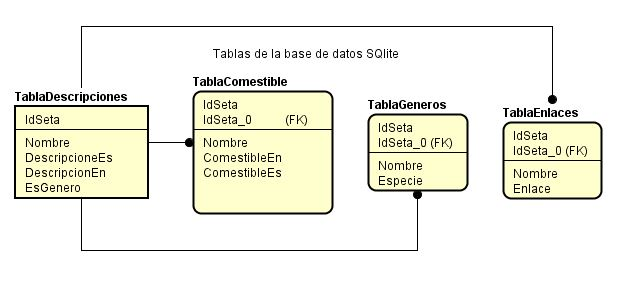
\includegraphics[width=1\textwidth]{imagenesAnexos/imagenesDiseno/TablasSQlite}%
          \caption{Tablas de la base de datos SQlite.}%
          \label{figTablasSQlite}%
        \end{center}%
  	\end{center}%
\end{figure}%

\begin{itemize}
	\item TablaComestible: Almacena la comestibilidad de una determinada especie en español e inglés.
	\item TablaDescripciones: Almacena la descripción de una determinada especie en español e inglés.
	\item TablaGeneros: Almacena el género al que pertenece una especie.
	\item TablaEnlaces: Almacena la url de la \textit{Wikipedia} de la especie. 
\end{itemize}

\subsection{Almacenamiento claves dicotómicas}

Las claves dicotómicas están guardadas en un archivo que contienen las siguientes estructuras java serializadas:

\begin{itemize}
	\item Map\textless String, ArrayList \textless String \textgreater \ \textgreater      arbolNodos : Este mapa contiene por cada género un arrayList con los siguientes tres mapas:
	\begin{itemize}
		\item Map\textless String, ArrayList\textless String\textgreater \ \textgreater arbolNodos: Mapa cuyas claves son los nodos y los valores son los nodos hijos de ese nodo padre. 
		
Este mapa nos sirve para contener la estructura de la clave.
		\item Map\textless String, ArrayList\textless String\textgreater \ \textgreater contenidoNodos: Mapa cuyas claves son los nodos y los valores son un array de Strings en el que la primera posición contienen la pregunta de ese nodo, la segunda posición es el enlace de esa especie, la tercera posición es el nodo padre y la cuarta posición contiene el género de esa especie.
		
Este mapa sirve para almacenar el contenido de cada nodo.
		\item Map\textless String, String\textgreater generosNodos: Mapa en el que las claves son géneros y los hijos son el nodo que contiene ese género dentro del mapa contenidoNodos.
		
Este mapa facilita acceder al nodo que contiene el género buscado de seta.
	\end{itemize}
\end{itemize}

\subsection{Diagramas de clases}
\subsubsection{Diagramas de clases del proyecto de Eclipse}

En la figura \ref{figDiagramaClasesJava} podemos observar las clases implementadas en el proyecto de Eclipse y que dependencias tienen entre sí. A continuación se muestra una breve descripción de la funcionalidad de cada clase y el paquete en el que esta contenida.

Para acceder a una descripción de los métodos acceder al \textbf{javadoc} de cada proyecto.

\begin{itemize}
	\item Paquete \textit{basedatossql}: Contiene las clases necesarias para crear y manejar la base de datos SQlite.
	\begin{itemize}
		\item Clase \textit{BDsql}: Clase que contiene los Métodos necesarios para acceder a una base de datos SQlite y manejarla.
		\item Clase \textit{CreadorBD}: Clase que crea la base de datos a partir de BDsql y DBpedia.
	\end{itemize}
	\item Paquete \textit{creador}: Contiene la clase que contiene el \textit{main} del proyecto.
	\begin{itemize}
		\item Clase \textit{CreadorBDyClaves}: Clase que lanza los métodos necesarios para crear la base de datos y extraer las claves dicotómicas.
	\end{itemize}
	\item Paquete \textit{dbpedia}: Contiene las clases necesarias para extraer la información de la DBpedia.
	\begin{itemize}
		\item Clase \textit{DBpedia}: Clase que contiene los métodos necesarios realizar consultas a la web semántica DBpedia.
	\end{itemize}
	\item Paquete \textit{traductor}: Contiene las clases necesarias para implementar un traductor automático.
	\begin{itemize}
		\item Clase \textit{Translator}: Clase que permite traducir cualquier texto a través de llamadas al traductor de Google. Clase descargada de \href{http://archana-testing.blogspot.com.es/2016/02/calling-google-translation-api-in-java.html}{\textit{archana-testing.}}
	\end{itemize}
	\item Paquete \textit{webscraping}: Contiene las clases necesarias realizar la extracción de las claves dicotómicas mediante técnicas de \textit{Web Scraping}.
	\begin{itemize}
		\item Clase \textit{ClaveDicotomica}: Clase que guarda la estructura de una clave dicotómica y tiene los métodos para cargarla de la url proporcionada y acceder a sus elementos. Esta preparada para funcionar con las claves de la página web \url{http://www.avelinosetas.info}
		\item Clase \textit{CreadorClaves}: Clase que contiene los métodos necesarios para serializar las claves dicotómicas.
	\end{itemize}
\end{itemize}
\begin{figure}[h]
    \begin{center}%
        \begin{center}%
          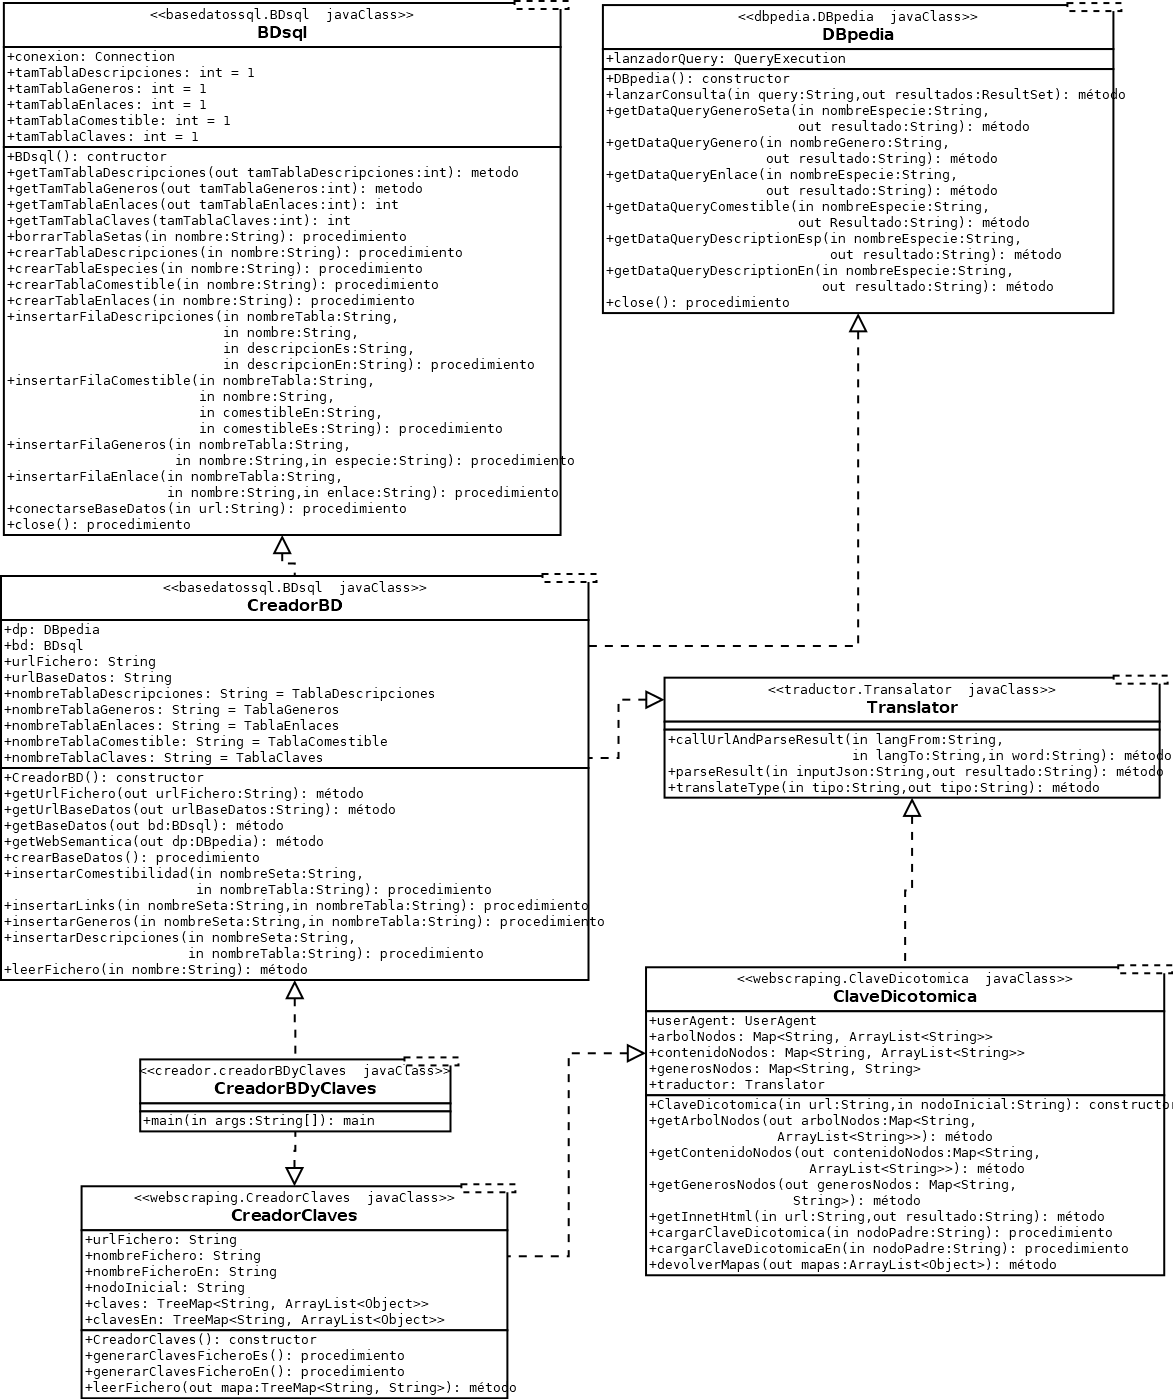
\includegraphics[width=1\textwidth]{imagenesAnexos/imagenesDiseno/DiagramaClasesJava}%
          \caption{Diagrama de clases del proyecto de Eclipse.}%
          \label{figDiagramaClasesJava}%
        \end{center}%
  	\end{center}%
\end{figure}%

\newpage
\subsubsection{Diagramas de clases del proyecto Android}

En esta sección se van a detallar los diagramas de clases del proyecto Android.

Para acceder a una descripción de los métodos acceder al \textbf{javadoc} de cada proyecto.

\begin{itemize}

	%1-PAQUETE BASEDATOS
	
	\item Paquete \textit{basedatos}: Paquete que contiene todas las clases necesarias para acceder a los datos de la aplicación. Diagrama de clases en la figura \ref{figDiagramaClasesAndroidBaseDatos}.
	\begin{itemize}
		\item Clase \textit{AccesoDatosExternos}: Clase que implementa las funciones necesarias para acceder a los datos externos a la aplicación que se encuentran en la carpeta assets.
		\item Clase \textit{DBsetas}: Clase que carga la base de datos SQLite encontrada en assets/databases.
		\item Clase \textit{DBsetasManager}: Clase que implementa los métodos para acceder y administrar la base de datos.
	\end{itemize}
	
	%2-PAQUETE CLASIFICADOR
	
	\item Paquete \textit{clasificador}: Paquete que contiene las clases y actividades relacionadas con la implementación y uso del clasificador de imágenes. Diagrama de clases en la figura \ref{figDiagramaClasesAndroidClasificador}.
	\begin{itemize}
		\item Clase \textit{RecogerFoto}: Clase que implementa la funcionalidad relacionada con la toma y guardado de fotografías.
		\item Clase \textit{TensorFlowImageClassifier}: Clase implementada por Tensorflow que permite usar un clasificador entrenado en Android.
	\end{itemize}
	
	%3-PAQUETE CLAVEDICOTOMICA
	
	\item Paquete \textit{clavedicotomica}: Paquete que contiene las clases relacionadas con mostrar las claves dicotómicas. Diagrama de clases en la figura \ref{figDiagramaClasesAndroidClaveDicotomica}.
	\begin{itemize}
		\item Clase \textit{ClaveDicotomica}: Clase que implementa la funcionalidad relacionada con mostrar la clave dicotómica seleccionada.
		\item Clase \textit{MostrarClaves}: Clase que muestra un listado de las claves dicotómicas de la aplicación.
	\end{itemize}
	
	%4-PAQUETE ELEGIRCLAVES
	
	\item Paquete \textit{elegirclaves}: Paquete que contiene las clases relacionadas con el filtrado de géneros de la clave general. Diagrama de clases en la figura \ref{figDiagramaClasesAndroidElegirClaves}.
	\begin{itemize}
		\item Clase \textit{AdaptadorSelector}: Clase que implementa el adaptador para cargar los elementos (ItemSelector) de la lista de géneros a seleccionar.
		\item Clase \textit{ViewHolderSelector}: Clase que implementa los elementos que se deben cargar en la lista (selector)y los relaciona con los elementos de la interfaz.
		\item Clase \textit{ElegirClaves}: Clase que muestra los géneros a elegir para filtrar la clave dicotómica general.
		\item Clase \textit{ItemSelector}: Clase que implementa los elementos del selector.
	\end{itemize}
	
	%5-PAQUETE INFORMACION
	
	\item Paquete \textit{informacion}: Paquete que contiene las clases relacionadas con mostrar la información de las distintas especies manejadas por la aplicación. Diagrama de clases en la figura \ref{figDiagramaClasesAndroidInformacion}.
	\begin{itemize}
		\item Clase \textit{MostrarSetas}: Clase que muestra las setas de la aplicación mediante un listado de tipo RecyclerView.
		\item Clase \textit{MostrarInformacionSetas}: Clase que muestra información relativa a la seta pulsada.
	\end{itemize}
	
	%6-PAQUETE LANZADOR
	
	\item Paquete \textit{lanzador}: Paquete que recoge la clase lanzadora de la aplicación. Diagrama de clases en la figura \ref{figDiagramaClasesAndroidLanzador}.
	\begin{itemize}
		\item Clase \textit{Lanzadora}: Clase que arranca la aplicación. Muestra los botones principales para acceder a las funcionalidades más importantes de la aplicación.
	\end{itemize}
	
	%7-PAQUETE RESULTADOS
	
	\item Paquete \textit{resultados}: Paquete que contiene las clases relacionadas con mostrar los resultados obtenidos por el clasificador. Diagrama de clases en la figura \ref{figDiagramaClasesAndroidResultados}.
	\begin{itemize}
		\item Clase \textit{AdaptadorSetasLista}:Clase que sirve de adaptador al sistema para cargar en cada elemento de la lista una foto y el nombre de la especie de la seta.
		\item Clase \textit{SetasListaHolder}: Clase que contiene cada par imagenView-TextView de cada elemento de la lista.
		\item Clase \textit{SetasLista}: Clase que implementa el contenido que va a tener la lista de imágenes que se muestran como resultado tras clasificar una foto.
		\item Clase \textit{MostrarComparativa}: Clase que muestra la foto introducida por el usuario y la seleccionada.
		\item Clase \textit{MostrarResultados}: Clase que implementa la funcionalidad de la actividad que muestra los resultados obtenidos tras
clasificar una foto.
	\end{itemize}
	
	%8-PAQUETE TARJETASCLAVES
	
	\item Paquete \textit{tarjetasclaves}: Paquete que contiene las clases relacionadas con mostrar el listado de claves dicotómicas disponibles en la aplicación. Diagrama de clases en la figura \ref{figDiagramaClasesAndroidTarjetasClaves}.
	\begin{itemize}
		\item Clase \textit{AdaptadorTarjetasClaves}: Clase que implementa el adaptador para cargar los elementos de la lista de las claves dicotómicas.
		\item Clase \textit{ViewHolder}: Clase que implementa los elementos que se deben cargar en la lista de claves.
		\item Clase \textit{TarjetaClave}: Clase que implementa el contenido de una tarjeta de claves dicotómicas.
	\end{itemize}
	
	%9-PAQUETE TARJETASCLAVES
	
	\item Paquete \textit{tarjetassetas}: Paquete que contiene las clases relacionadas con mostrar el listado de especies disponibles en la aplicación. Diagrama de clases en la figura \ref{figDiagramaClasesAndroidTarjetasSetas}.
	\begin{itemize}
		\item Clase \textit{AdaptadorTarjetasSetas}: Clase que implementa el adaptador para cargar los elementos de la lista de setas.
		\item Clase \textit{ViewHolder}: Clase que implementa los elementos que se deben cargar en la lista de setas.
		\item Clase \textit{TarjetaSeta}: Clase que implementa el contenido de una tarjeta de la lista de especies de setas.
	\end{itemize}
	
\end{itemize}

\newpage
%1
\begin{figure}[h]
    \begin{center}%
        \begin{center}%
          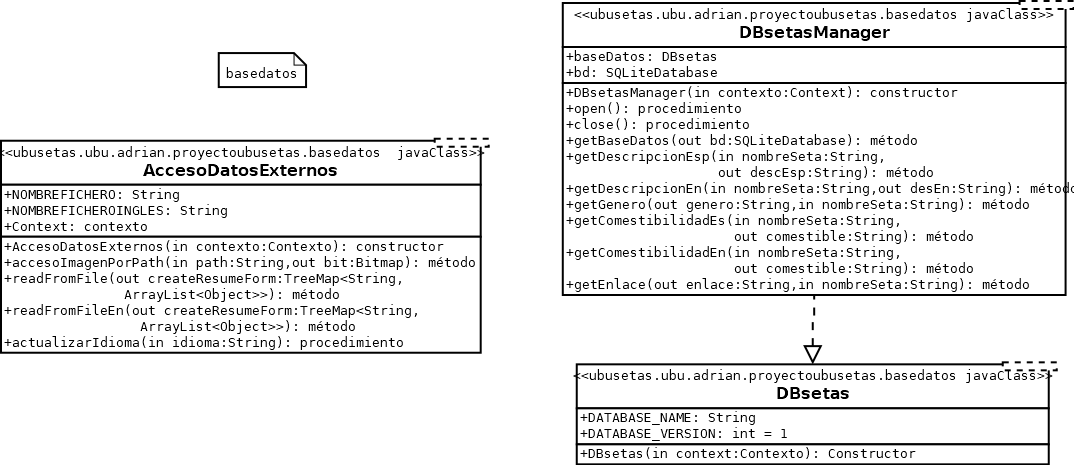
\includegraphics[width=1\textwidth]{imagenesAnexos/imagenesDiseno/DiagramaClasesAndroidBaseDatos}%
          \caption{Diagrama de clases del paquete basedatos.}%
          \label{figDiagramaClasesAndroidBaseDatos}%
        \end{center}%
  	\end{center}%
\end{figure}%
%2
\begin{figure}[h]
    \begin{center}%
        \begin{center}%
          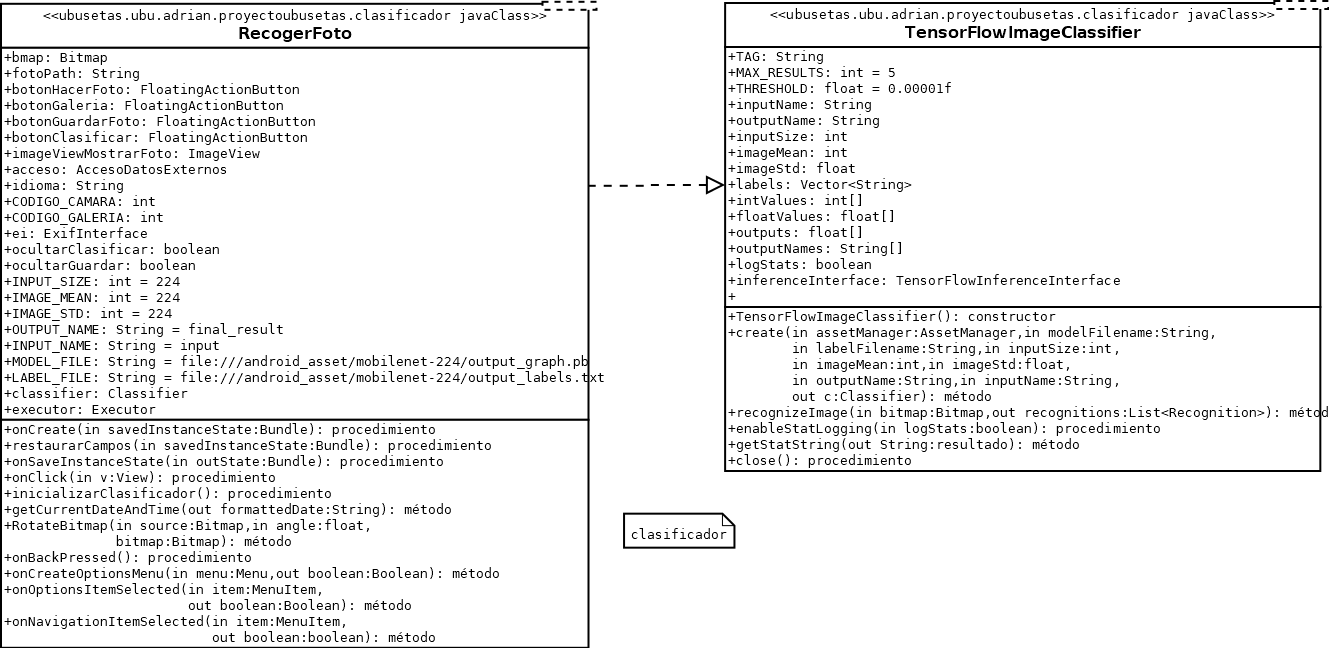
\includegraphics[width=1\textwidth]{imagenesAnexos/imagenesDiseno/DiagramaClasesAndroidClasificador}%
          \caption{Diagrama de clases del paquete clasificador.}%
          \label{figDiagramaClasesAndroidClasificador}%
        \end{center}%
  	\end{center}%
\end{figure}%
%3
\begin{figure}[h]
    \begin{center}%
        \begin{center}%
          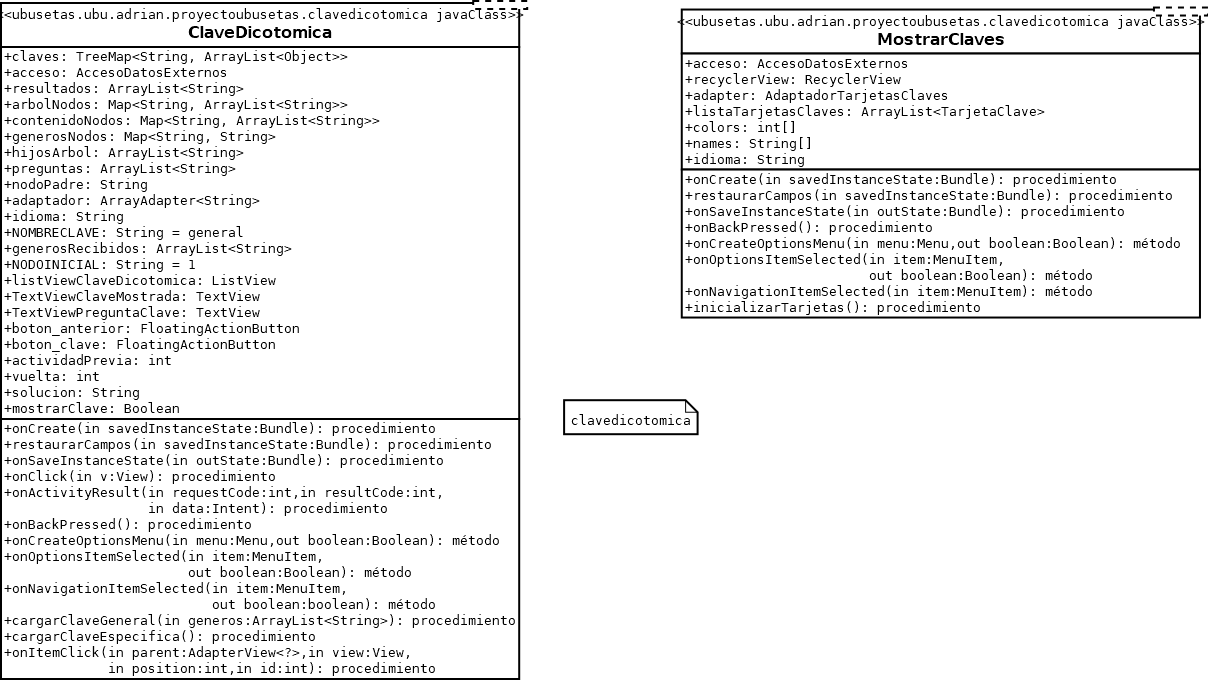
\includegraphics[width=1\textwidth]{imagenesAnexos/imagenesDiseno/DiagramaClasesAndroidClaveDicotomica}%
          \caption{Diagrama de clases del paquete clavedicotomica.}%
          \label{figDiagramaClasesAndroidClaveDicotomica}%
        \end{center}%
  	\end{center}%
\end{figure}%
%4
\begin{figure}[h]
    \begin{center}%
        \begin{center}%
          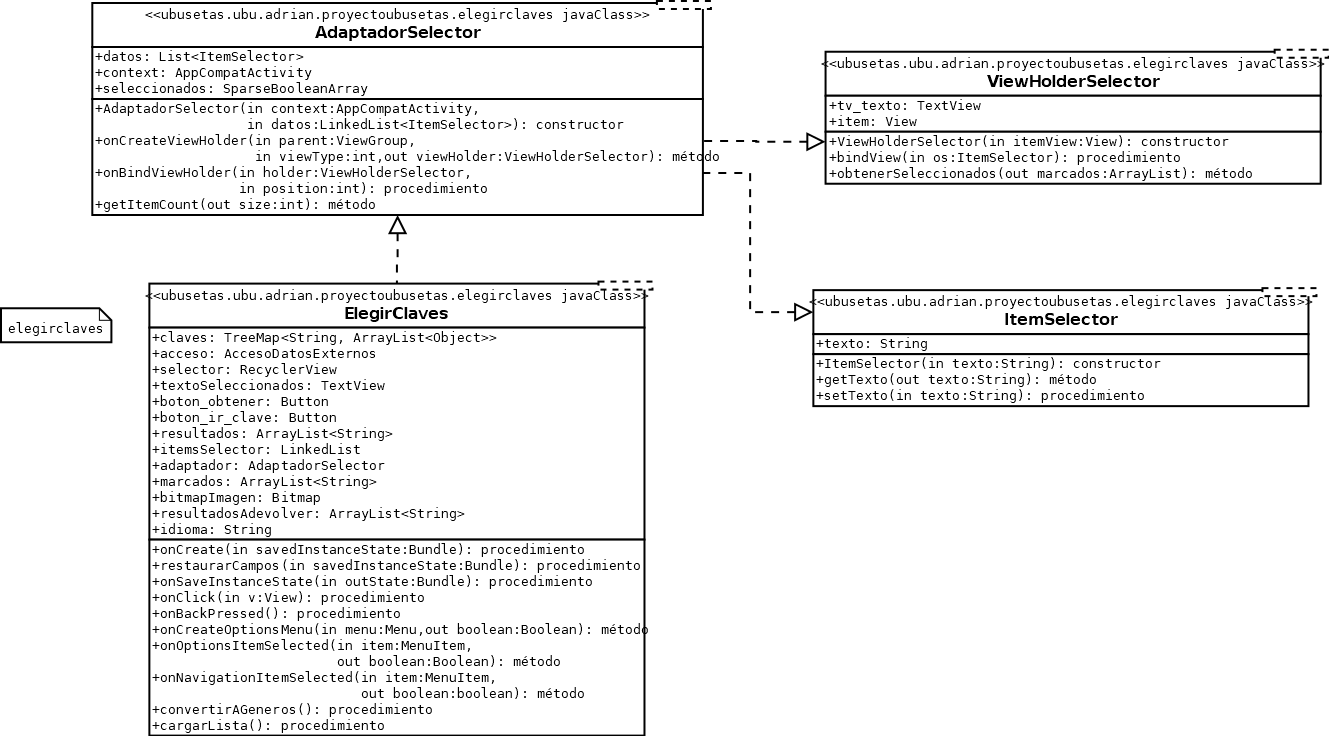
\includegraphics[width=1\textwidth]{imagenesAnexos/imagenesDiseno/DiagramaClasesAndroidElegirClaves}%
          \caption{Diagrama de clases del paquete elegirclaves.}%
          \label{figDiagramaClasesAndroidElegirClaves}%
        \end{center}%
  	\end{center}%
\end{figure}%
%5
\begin{figure}[h]
    \begin{center}%
        \begin{center}%
          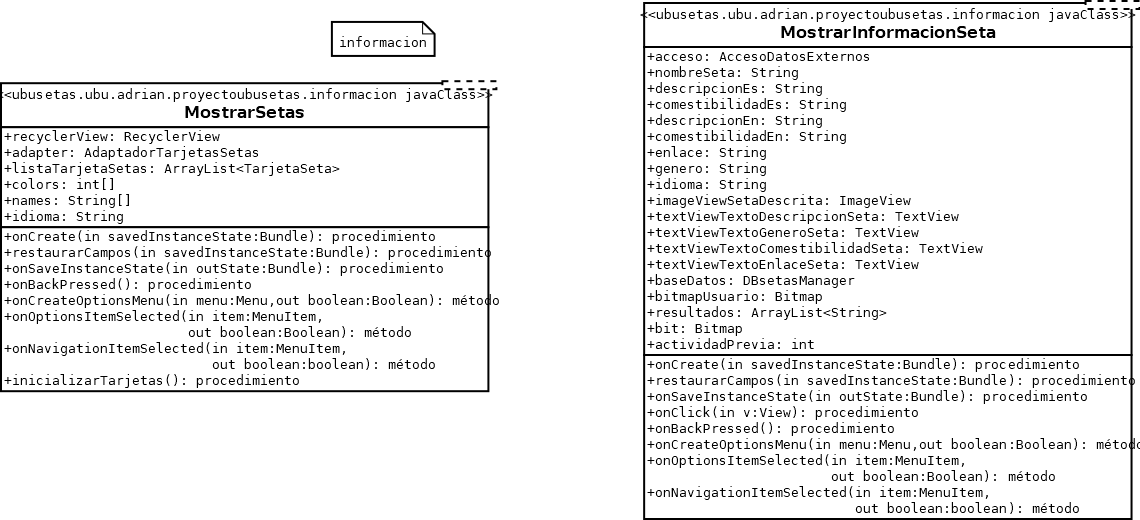
\includegraphics[width=1\textwidth]{imagenesAnexos/imagenesDiseno/DiagramaClasesAndroidInformacion}%
          \caption{Diagrama de clases del paquete informacion.}%
          \label{figDiagramaClasesAndroidInformacion}%
        \end{center}%
  	\end{center}%
\end{figure}%
%6
\begin{figure}[h]
    \begin{center}%
        \begin{center}%
          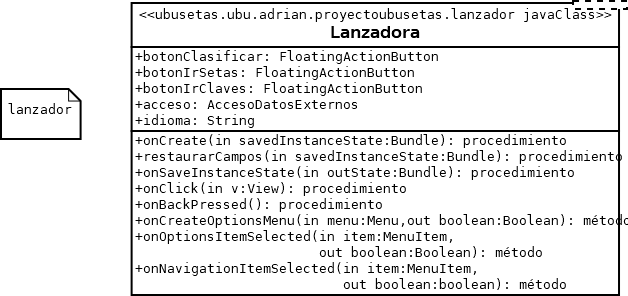
\includegraphics[width=1\textwidth]{imagenesAnexos/imagenesDiseno/DiagramaClasesAndroidLanzador}%
          \caption{Diagrama de clases del paquete lanzador.}%
          \label{figDiagramaClasesAndroidLanzador}%
        \end{center}%
  	\end{center}%
\end{figure}%
%7
\begin{figure}[h]
    \begin{center}%
        \begin{center}%
          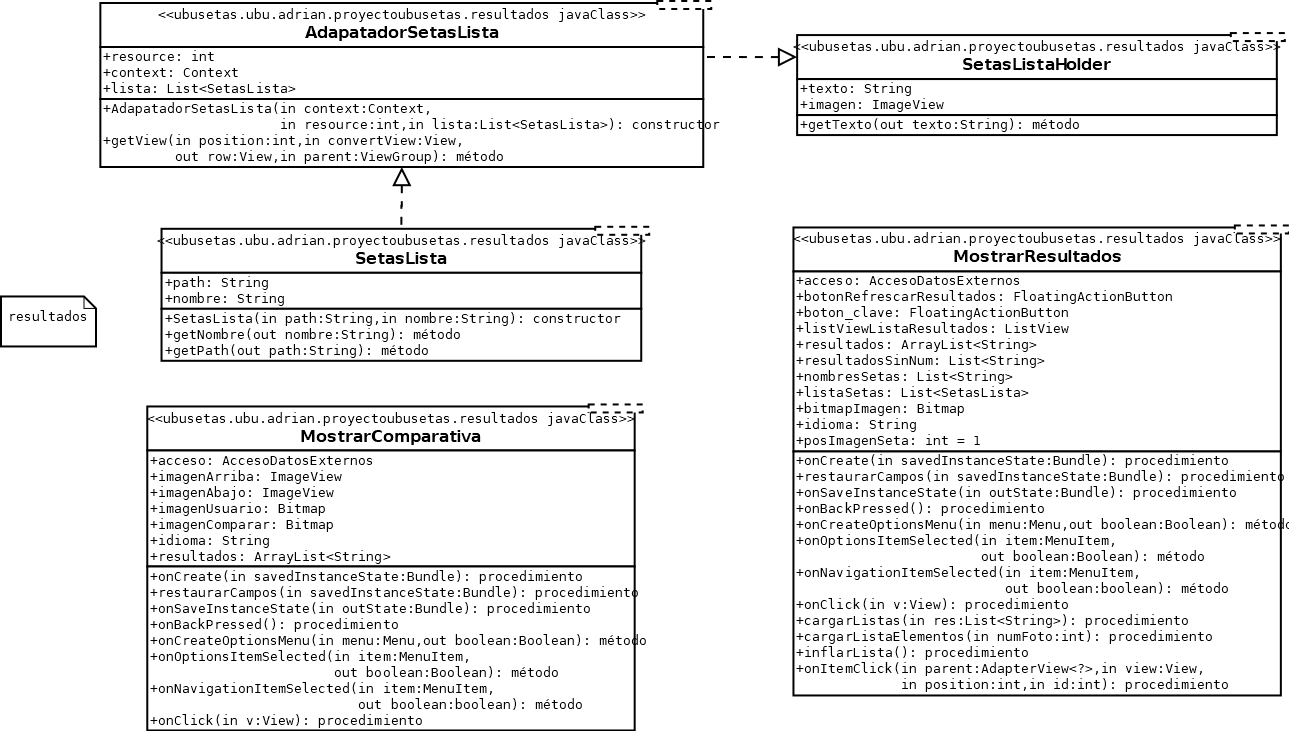
\includegraphics[width=1\textwidth]{imagenesAnexos/imagenesDiseno/DiagramaClasesAndroidResultados}%
          \caption{Diagrama de clases del paquete resultados.}%
          \label{figDiagramaClasesAndroidResultados}%
        \end{center}%
  	\end{center}%
\end{figure}%
%8
\begin{figure}[h]
    \begin{center}%
        \begin{center}%
          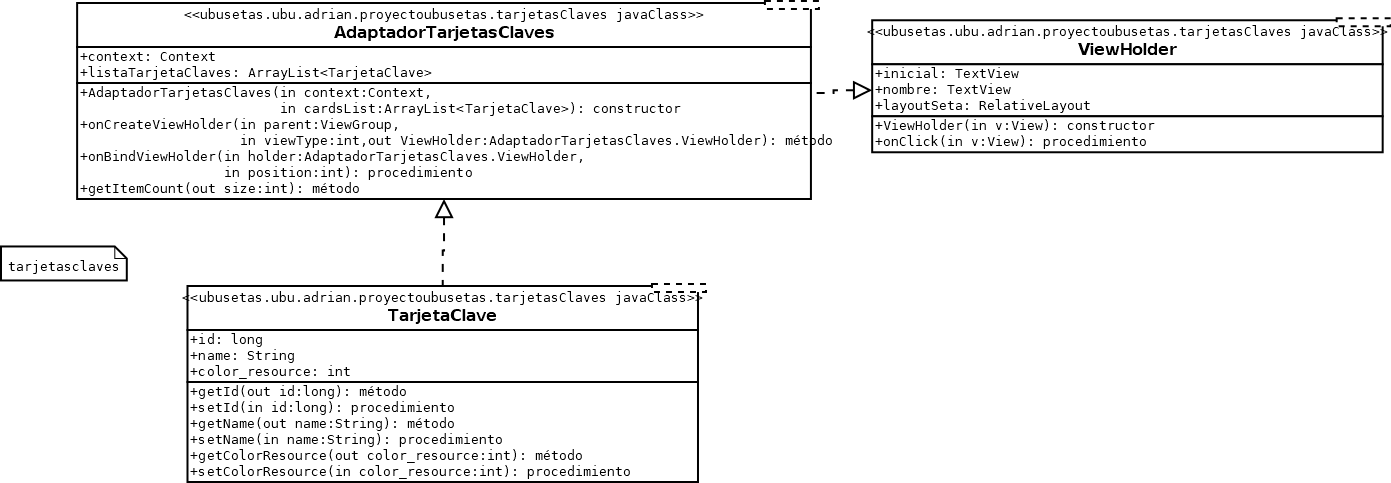
\includegraphics[width=1\textwidth]{imagenesAnexos/imagenesDiseno/DiagramaClasesAndroidTarjetasClaves}%
          \caption{Diagrama de clases del paquete tarjetasclaves.}%
          \label{figDiagramaClasesAndroidTarjetasClaves}%
        \end{center}%
  	\end{center}%
\end{figure}%
%9

\begin{figure}[h]
    \begin{center}%
        \begin{center}%
          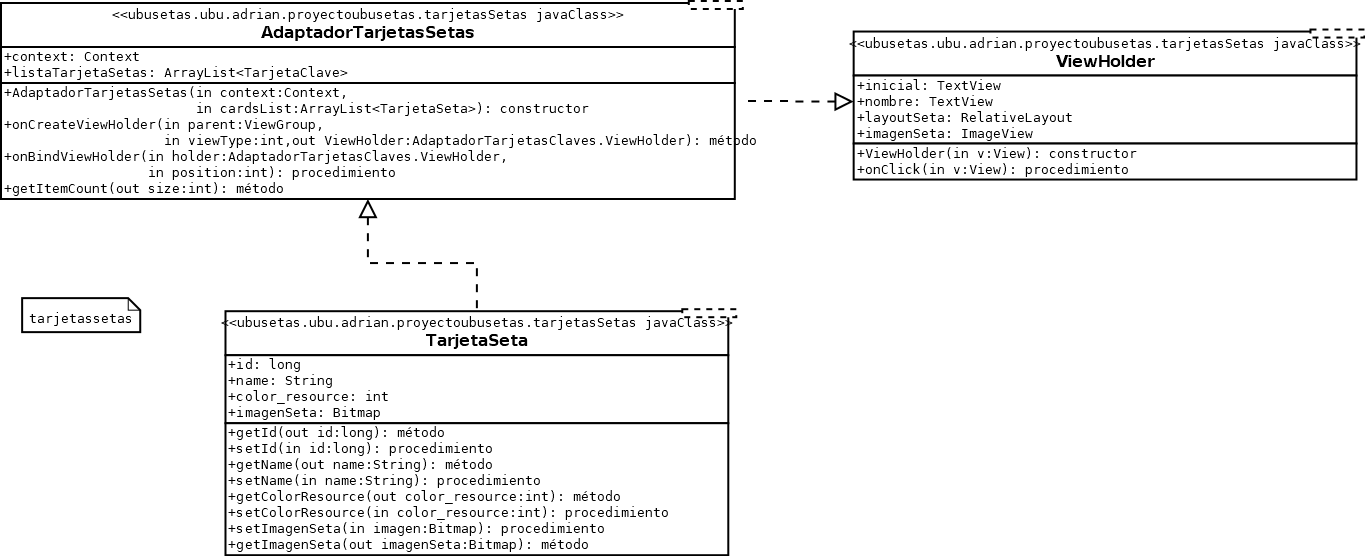
\includegraphics[width=1\textwidth]{imagenesAnexos/imagenesDiseno/DiagramaClasesAndroidTarjetasSetas}%
          \caption{Diagrama de clases del paquete tarjetassetas.}%
          \label{figDiagramaClasesAndroidTarjetasSetas}%
        \end{center}%
  	\end{center}%
\end{figure}%

\clearpage

\section{Diseño procedimental}

Sección en la que se van a explicar los pasos para realizar los procesos más relevantes de la aplicación Android.

\subsection{Clasificar imagen}

Para clasificar una imagen desde la aplicación Andrroi, el usuario deberá seguir estos pasos:

\begin{itemize}
	\item Paso 1: Iniciar la aplicación.
	\item Paso 2: Pulsar sobre el botón de \textit{clasificar} disponible en la actividad lanzadora o en el menú.
	\item Paso 3: Pulsar sobre el botón de galería o cámara disponibles en la siguiente actividad para cargar la imagen, bien desde la galería o desde la cámara de fotos del móvil.
	\item Paso 4: Introducir una imagen de una seta.
	\item Paso 5: En este momento, aparecerá el botón de clasificar. Pulsar sobre este botón.
	\item Paso 6: La aplicación mostrará un listado de las especies más probables clasificadas para esa imagen.
\end{itemize}

\subsection{Selección de géneros para usar la clave dicotómica}

Una vez el usuario haya clasificado una imagen, podrá acceder a una clave dicotómica filtrada según los resultados obtenidos. El usuario podrá elegir los géneros de setas sobre los que aplicar la clave, si lo desea podrá aplicarla sobre todos los disponibles.

\begin{itemize}
	\item Paso 1: Realizar los pasos del procedimiento \textit{Clasificar imagen}.
	\item Paso 2: Pulsar sobre el botón de acceso a la clave dicotómica.
	\item Paso 3: Seleccionar de la lista los géneros deseados. Para ello primero se eligen los géneros pulsando sobre ellos y después se pulsa sobre el botón de seleccionar.
	\item Paso 4: Pulsar sobre el botón \textit{ir clave dicotómica}.
	\item Paso 5: En este momento, se mostrarán las preguntas relacionadas con los géneros seleccionados.
\end{itemize}

\subsection{Seleccionar clave dicotómica}

El usuario podrá seleccionar una clave de las disponibles en la aplicación.

\begin{itemize}
	\item Paso 1: Iniciar la aplicación.
	\item Paso 2: Pulsar sobre el botón de \textit{ir claves} disponible en la actividad lanzadora o en el menú.
	\item Paso 3: Pulsar sobre la clave dicotómica del género de seta deseado.
	\item Paso 4: En este momento, se mostrarán las preguntas relacionadas con la clave seleccionada.
\end{itemize}
\subsection{Acceder a información de especie de seta}

El usuario podrá acceder a la información de una especie de seta recogida por la aplicación. Esta acción se podrá realizar de las siguientes dos formas:

\subsubsection{Forma 1}

\begin{itemize}
	\item Paso 1: Iniciar la aplicación.
	\item Paso 2: Pulsar sobre el botón de \textit{mostrar setas} disponible en la actividad lanzadora o en el menú.
	\item Paso 3: Pulsar sobre la especie de seta deseada.
	\item Paso 4: En este momento, se mostrará información describiendo la especie pulsada.
\end{itemize}

\subsubsection{Forma 2}

\begin{itemize}
	\item Paso 1: Realizar los pasos del procedimiento \textit{Clasificar imagen}.
	\item Paso 2: Mantener pulsado uno de los resultados
	\item Paso 3: En este momento, se mostrará información describiendo la especie pulsada.
\end{itemize}

\subsection{Responder una clave dicotómica}

El usuario podrá responder las preguntas de la clave dicotómica. Esta acción se podrá realizar de las siguientes dos formas:

\subsubsection{Forma 1}

\begin{itemize}
	\item Paso 1: Realizar los pasos del procedimiento \textit{Seleccionar clave dicotómica}.
	\item Paso 2: Ir respondiendo a las preguntas que va realizando la aplicación.
	\item Paso 3: El usuario podrá volver a la pregunta anterior pulsando el botón de volver.
	\item Paso 4: Una vez se hayan respondido todas las preguntas, se mostrará el género o especie clasificado por la clave, según esta sea la clave de géneros o una de especies.
	\item Paso 5: Si la aplicación tiene una clave dicotómica del género clasificado, se notificará al usuario y aparecerá un botón que le redirija a la clave que discrimina las especies de ese género.
\end{itemize}

\subsubsection{Forma 2}

\begin{itemize}
	\item Paso 1: Realizar los pasos del procedimiento \textit{Selección de géneros para usar la clave dicotómica}.
	\item Paso 2: Ir respondiendo a las preguntas que va realizando la aplicación.
	\item Paso 3: El usuario podrá volver a la pregunta anterior pulsando el botón de volver.
	\item Paso 4: Una vez se hayan respondido todas las preguntas, se mostrará el género clasificado por la clave
	\item Paso 5: Si la aplicación tiene una clave dicotómica del género clasificado, se notificará al usuario y aparecerá un botón que le redirija a la clave que discrimina las especies de ese género.
\end{itemize}

\section{Diseño arquitectónico}

En esta sección se va a mostrar la estructura de paquetes seguida tanto en el proyecto Android como en el de Eclipse.

\subsection{Proyecto Eclipse}

A continuación se muestra una descripción de los paquetes del proyecto de Eclipse y como se relacionan entre sí.

\begin{itemize}
	\item Paquete \textit{basedatossql}: Contiene las clases necesarias para crear y manejar la base de datos SQlite.
	\item Paquete \textit{creador}: Contiene la clase que contiene el \textit{main} del proyecto. Hace uso de los paquetes dbpedia y webscraping para extraer toda la información necesaria por la aplicación.
	\item Paquete \textit{dbpedia}: Contiene las clases necesarias para extraer la información de la DBpedia. Hace uso del paquete traductor para traducir al inglés la información. Hace uso del paquete basededatossql para almacenar la información consultada en la base de datos.
	\item Paquete \textit{traductor}: Contiene las clases necesarias para implementar un traductor automático.
	\item Paquete \textit{webscraping}: Contiene las clases necesarias realizar la extracción de las claves dicotómicas mediante técnicas de \textit{Web Scraping}.Hace uso del paquete traductor para traducir las claves dicotómicas.
\end{itemize}

En la figura \ref{figDiagramaPaquetesJava} se muestra el diagrama de paquetes del proyecto de Eclipse.

\begin{figure}[h]
    \begin{center}%
        \begin{center}%
          \includegraphics[width=1\textwidth]{imagenesAnexos/imagenesDiseno/DiagramaPaquetesJava}%
          \caption{Diagrama de paquetes del proyecto de Eclipse.}%
          \label{figDiagramaPaquetesJava}%
        \end{center}%
  	\end{center}%
\end{figure}%

\newpage
\subsection{Proyecto Android}

A continuación se muestra una descripción de los paquetes del proyecto Android y como se relacionan entre sí.

\begin{itemize}

	%1-PAQUETE BASEDATOS
	
	\item Paquete \textit{basedatos}: Paquete que contiene todas las clases necesarias para acceder a los datos de la aplicación.
	
	%2-PAQUETE CLASIFICADOR
	
	\item Paquete \textit{clasificador}: Paquete que contiene las clases y actividades relacionadas con la implementación y uso del clasificador de imágenes.
	
	%3-PAQUETE CLAVEDICOTOMICA
	
	\item Paquete \textit{clavedicotomica}: Paquete que contiene las clases relacionadas con mostrar las claves dicotómicas. Hace uso del paquete base de datos para extraer las claves dicotómicas del fichero serializado. Usa el paquete tarjetasclaves para implementar el listado de claves.
	
	%4-PAQUETE ELEGIRCLAVES
	
	\item Paquete \textit{elegirclaves}: Paquete que contiene las clases relacionadas con el filtrado de géneros de la clave general. 
	
	%5-PAQUETE INFORMACION
	
	\item Paquete \textit{informacion}: Paquete que contiene las clases relacionadas con mostrar la información de las distintas especies manejadas por la aplicación. Hace uso del paquete basedatos para extraer la información de la base de datos SQlite y acceder a las imágenes de las setas, situadas en los directorios externos. Usa el paquete tarjetassetas para implementar el listado de especies de setas.
	
	%6-PAQUETE LANZADOR
	
	\item Paquete \textit{lanzador}: Paquete que recoje la clase lanzadora de la aplicación.
	
	%7-PAQUETE RESULTADOS
	
	\item Paquete \textit{resultados}: Paquete que contiene las clases relacionadas con mostrar los resultados obtenidos por el clasificador. Hace uso del paquete basedatos para acceder a las imágenes de las setas, situadas en los directorios externos.
	
	%8-PAQUETE TARJETASCLAVES
	
	\item Paquete \textit{tarjetasclaves}: Paquete que contiene las clases relacionadas con mostrar el listado de claves dicotómicas disponibles en la aplicación.
	
	%9-PAQUETE TARJETASCLAVES
	
	\item Paquete \textit{tarjetassetas}: Paquete que contiene las clases relacionadas con mostrar el listado de especies disponibles en la aplicación.
	
\end{itemize}

En la figura \ref{figDiagramaPaquetesAndroid} se muestra el diagrama de paquetes del proyecto Android. 
\begin{figure}[h]
    \begin{center}%
        \begin{center}%
          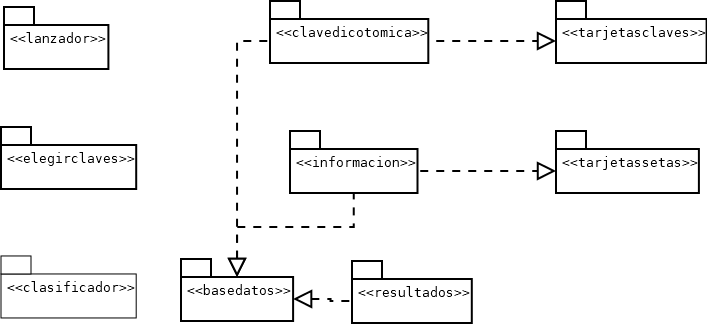
\includegraphics[width=1\textwidth]{imagenesAnexos/imagenesDiseno/DiagramaPaquetesAndroid}%
          \caption{Diagrama de paquetes del proyecto Android.}%
          \label{figDiagramaPaquetesAndroid}%
        \end{center}%
  	\end{center}%
\end{figure}%

\section{Diseño de la interfaz}

En esta sección se van a explicar los pasos seguidos para implementar la interfaz de la aplicación Android.

\subsection{Prototipado}

El prototipado de la aplicación se realizó de manera manual, dibujando un diseño inicial de lo que iba a ser la interfaz de cada actividad. A continuación se muestran las tarjetas de las diferentes actividades.
\apendice{Documentación técnica de programación}

\section{Introducción}

Sección en la que se va a explicar la estructura de directorios que sigue la entrega del proyecto y a continuación, se desarrollarán los pasos necesarios para compilar y ejecutar los componentes del proyecto. El objetivo de esta sección es mostrar los pasos que se deben seguir para instalar todos los componentes necesarios para seguir desarrollando este proyecto.

\section{Estructura de directorios}

A continuación se van a listar los directorios que forman este proyecto y que están en el directorio raíz.

\begin{itemize}
	\item \textbf{\textbackslash Proyecto Eclipse:} Esta carpeta contiene los códigos fuente de la aplicación de Eclipse, el nombre del proyecto es \textit{ExtraccionDatos}.
	
	\item \textbf{\textbackslash Proyecto Android:} Esta carpeta contiene los códigos fuente de la aplicación Android, el nombre del proyecto es \textit{ProyectoUbusetas}.
	
	\item \textbf{\textbackslash Herramientas adicionales:} Contiene las librerías y proyectos externos \textit{open source} usados en este proyecto. 
	
	\begin{itemize}
	 	\item \textbf{\textbackslash Herramientas adicionales\textbackslash \textit{image\_retraining}:} Esta carpeta contiene el proyecto de \textit{Tensorflow} usado para entrenar los clasificadores de imágenes.
	 	\item \textbf{\textbackslash Herramientas adicionales\textbackslash apache-jena-3.4.0:} Las librerías de Apache Jena.
	 	\item \textbf{\textbackslash Herramientas adicionales\textbackslash jaunt1.3.7:} Las librerías de Apache Jaunt.
	 	\item \textbf{\textbackslash Herramientas adicionales\textbackslash json-20171018:} Las librerías de Json.
	 	\item \textbf{\textbackslash Herramientas adicionales\textbackslash sqlite-jdbc-3.20.0:} El driver de la base de datos SQlite.
	\end{itemize}
	 
	\item \textbf{\textbackslash Git:} Contiene una copia del repositorio de Github del proyecto.
	 
	\item \textbf{\textbackslash Documentación:} Contiene la documentación del proyecto, esta carpeta contiene los siguientes elementos:
	\begin{itemize}
		\item \textbf{\textbackslash Documentación\textbackslash memoria.pdf:} La memoria del proyecto.
	 	\item \textbf{\textbackslash Documentación\textbackslash anexos.pdf:} Los anexos del proyecto.
	 	\item \textbf{\textbackslash Documentación\textbackslash fuentes latex:} Carpeta con los códigos de latex usados para generar la documentación.
	\end{itemize}
	 
	\item \textbf{\textbackslash Documentación adicional:} Contiene las siguientes dos carpetas con los \textit{javadoc} de los proyectos.
	\begin{itemize}
	 	\item \textbf{\textbackslash Documentación adicional\textbackslash javadoc proyecto Eclipse:} Esta carpeta contiene la documentación del proyecto Eclipse.
	 	\item \textbf{\textbackslash Documentación adicional\textbackslash javadoc proyecto Android:} Esta carpeta contiene la documentación del proyecto Android.
	\end{itemize}
	 
	\item \textbf{\textbackslash Binarios\textbackslash aplicación Android:} Carpeta donde se encuentra el instalador de la aplicación Android llamado \textit{UBUsetas1.0.apk}
	 
	\item \textbf{\textbackslash Tutoriales:} Contiene tutoriales para instalar ciertas herramientas y librerías necesarias para el funcionamiento del proyecto.
	
\end{itemize}

\section{Manual del programador}

Manual donde se va a explicar como realizar las tareas que llevaría a cabo el desarrollador o administrador de la aplicación.

\subsection{Realización de las consultas a la DBpedia}

En este apartado se van a explicar los pasos que hay que seguir para descargar la información de las especies de setas, a través del proyecto de Eclipse, y almacenarlas en una base de datos SQlite para su posterior exportación a la aplicación Android.

Para realizar esta tarea es necesario haber creado antes una base de datos \textit{SQlite}. En la carpeta \textbackslash Tutoriales se encuentra el pdf llamado "\textit{Instalación SQlite windows"} en el que se explica como instalar y crear una base de datos \textit{SQlite}.

Una vez tengamos la base de datos, deberemos especificar al programa la ruta donde se encuentra. Para ello editamos la clase \textit{CreadorBD.java} indicándole en la siguiente línea \ref{figRutaBaseDatos} la ruta.

\begin{figure}[h]
    \begin{center}%
        \begin{center}%
          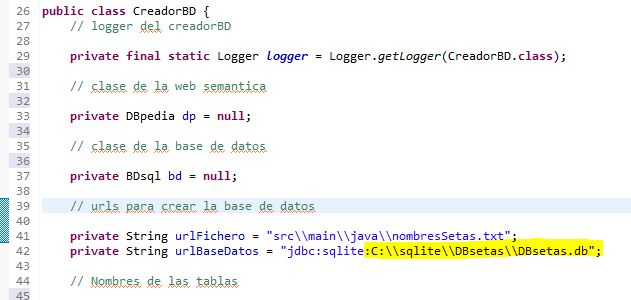
\includegraphics[width=1\textwidth]{imagenesAnexos/imagenesManualProgramador/RutaBaseDatos}%
          \caption{Ruta de la base de datos.}%
          \label{figRutaBaseDatos}%
        \end{center}%
  	\end{center}%
\end{figure}%

Una vez hecho esto, deberemos ejecutar el \textit{main} que encontramos en la clase \textit{src/main/java/dbpedia/DBpedia.java}. El programa realizará las consultas a la \textit{DBpedia} y guardará la información de las especies en la base de datos \textit{SQlite} especificada. Este proceso tardará unos minutos, dependiendo de la velocidad de la conexión a Internet.

La lista de especies de setas a consultar se encuentra en el fichero que encontramos en la ruta \textit{src/main/java/nombresSetas.txt} del proyecto.
Encontraremos la siguiente estructura \ref{figListaEspeciesSetas} en la que podremos añadir o quitar especies para consultar a la DBpedia. 

\begin{figure}[h]
    \begin{center}%
        \begin{center}%
          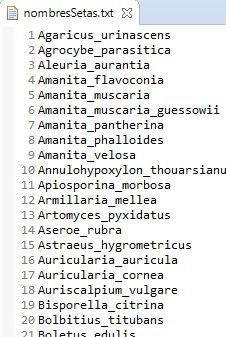
\includegraphics[width=0.5\textwidth]{imagenesAnexos/imagenesManualProgramador/ListaEspeciesSetas}%
          \caption{Listado de especies de setas.}%
          \label{figListaEspeciesSetas}%
        \end{center}%
  	\end{center}%
\end{figure}%

Por último, para instalar la base de datos en la aplicación Android, deberemos copiar nuestro fichero \textit{DBsetas.db} (o el nombre que le hayamos dado) dentro de la carpeta \textit{/app/src/main/assets/databases} del proyecto Android.
\clearpage

\subsection{Extracción de las claves dicotómicas}

En esta sección se explicará como ejecutar el proyecto Eclipse para que extraiga las claves dicotómicas, mediante \textit{web scraping}, de la página web \url{http://www.avelinosetas.info/claves.php}.

Para realizar esta tarea, simplemente deberemos ejecutar el main que se encuentra en la clase \textit{src/main/java/webscraping/ClaveDicotomica.java} del proyecto de Eclipse.

Una vez hayamos ejecutado este programa, se nos habrán creado dos archivos en la raíz del proyecto:
\begin{itemize}
	\item claves.dat: contiene las claves dicotómicas en Español.
	\item clavesEn.dat: contiene las claves dicotómicas en Inglés.
\end{itemize}

Por último, para instalar las claves en la aplicación Android, deberemos copiar nuestros ficheros \textit{claves.dat} y \textit{clavesEn.dat} dentro de la carpeta \textit{/app/src/main/assets/claves} del proyecto Android.

\subsection{Entrenamiento del clasificador}

En este apartado se explicará como usar el proyecto de Tensorflow para entrenar nuestro propio clasificador de imágenes. Este proyecto lo podremos encontrar en la carpeta \textbackslash Herramientas adicionales\textbackslash \textit{image\_retraining}. Tiene la siguiente estructura \ref{figEstructuraImageRetraining}.

\begin{figure}[h]
    \begin{center}%
        \begin{center}%
          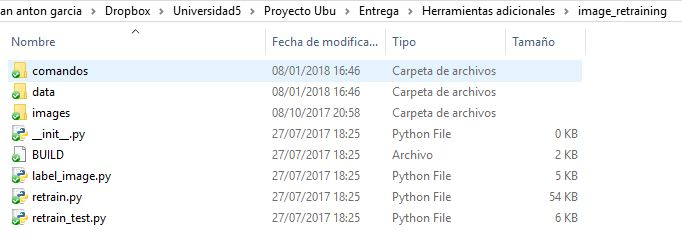
\includegraphics[width=1\textwidth]{imagenesAnexos/imagenesManualProgramador/EstructuraImageRetraining}%
          \caption{Estructura Image Retraining.}%
          \label{figEstructuraImageRetraining}%
        \end{center}%
  	\end{center}%
\end{figure}%

Para hacer uso de este proyecto necesitaremos tener instalados Python y Tensorflow\footnote{\url{https://www.tensorflow.org/install/}} en nuestro sistema.

Lo primero que deberemos hacer es colocar en la carpeta \textit{images} del proyecto nuestras imágenes divididas en carpetas. En cada carpeta colocaremos las imágenes que se correspondan con una misma especie de seta y 
llamaremos a esa carpeta con el nombre de la especie \ref{figListaEspeciesSetas}.

\begin{figure}[h]
    \begin{center}%
        \begin{center}%
          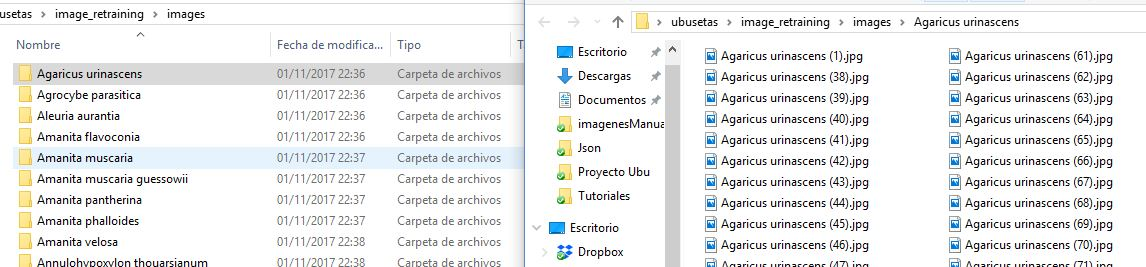
\includegraphics[width=1\textwidth]{imagenesAnexos/imagenesManualProgramador/ListadoEspeciesSetas}%
          \caption{Estructura Image Retraining.}%
          \label{figListadoEspeciesSetas}%
        \end{center}%
  	\end{center}%
\end{figure}%

Si queremos hacer uso del \textit{data augmentation}, deberemos modificar los parámetros dentro del fichero retrain.py, según se indica en las descripciones de estos dentro del código.

Para entrenar el modelo deberemos abrir una consola y colocarnos en la carpeta \textit{image\_retraining}. Una vez aquí deberemos activar Tensorflow con el siguiente comando \ref{figActivacionTensorflow}.

\begin{figure}[h]
    \begin{center}%
        \begin{center}%
          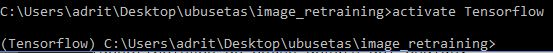
\includegraphics[width=1\textwidth]{imagenesAnexos/imagenesManualProgramador/ActivacionTensorflow}%
          \caption{Activación Tensorflow.}%
          \label{figActivacionTensorflow}%
        \end{center}%
  	\end{center}%
\end{figure}%

Cuando hayamos activado \textit{Tensorflow} podremos ejecutar el fichero retrain.py para entrenar el modelo. Deberemos especificarle el modelo que queremos entrenar, por ejemplo, para entrenar el \textit{Mobilenet-224} ejecutaríamos el siguiente comando \ref{figEntrenamientoTensorflow}.

\begin{figure}[h]
    \begin{center}%
        \begin{center}%
          \includegraphics[width=1\textwidth]{imagenesAnexos/imagenesManualProgramador/EntrenamientoTensorflow}%
          \caption{Entrenamiento Mobilenet.}%
          \label{figEntrenamientoTensorflow}%
        \end{center}%
  	\end{center}%
\end{figure}%
\newpage
Cuando el proceso acabe (puede tardar horas o días según la configuración), se nos generarán los siguientes dos archivos en la carpeta C:\textbackslash tmp:

\begin{itemize}
	\item output\_graph.pb: El modelo entrenado.
	\item output\_labels.txt: Los \textit{labels} del modelo.
\end{itemize}

Para instalar nuestro modelo Mobilenet en la aplicación Android deberemos colocar estos dos archivos en la carpeta \textit{/app/src/main/assets/mobilenet-224} del proyecto Android.

\section{Compilación, instalación y ejecución del proyecto}

En esta sección se desarrollarán los pasos necesarios para instalar tanto el proyecto Eclipse como el proyecto Android.

\subsection{Proyecto Eclipse}

En este apartado se explicará como instalar el proyecto de Eclipse llamado \textit{ExtraccionDatos}. Este proyecto lo podemos encontrar en la carpeta \textit{Proyecto Eclipse}, deberemos extraerlo para poder importarlo.

En el proyecto se ha usado la versión de Eclipse Neon.3 Release (4.6.3). Necesitaremos una versión de Eclipse\footnote{\url{http://www.eclipse.org/downloads/eclipse-packages/}} igual o superior a esta para instalarlo. Además necesitaremos tener instalado Maven en Eclipse\footnote{\url{https://maven.apache.org/install.html}}.

Para instalar el proyecto \textit{ExtraccionDatos} deberemos importarlo como un proyecto Maven de la siguiente forma \ref{figImportacionEclipse} \ref{figImportacionEclipse2}.

\begin{figure}[h]
    \begin{center}%
        \begin{center}%
          \includegraphics[width=0.6\textwidth]{imagenesAnexos/imagenesManualProgramador/ImportacionEclipse}%
          \caption{Importación Eclipse.}%
          \label{figImportacionEclipse}%
        \end{center}%
  	\end{center}%
\end{figure}%

\begin{figure}[h]
    \begin{center}%
        \begin{center}%
          \includegraphics[width=0.6\textwidth]{imagenesAnexos/imagenesManualProgramador/ImportacionEclipse2}%
          \caption{Importación Eclipse.}%
          \label{figImportacionEclipse2}%
        \end{center}%
  	\end{center}%
\end{figure}%

\clearpage
Una vez importado el proyecto base deberemos importar las siguientes librerías al proyecto. Se ha creado un tutorial para cada una que muestra como se descargan e importan al proyecto.

\begin{itemize}
	\item apache-jena-3.4.0: Es la librería que nos proporciona los métodos necesarios para realizar las consultas a la DBpedia. El tutorial se encuentra en el archivo \textit{Tutoriales/Instalación librería Jena en Eclise.pdf}.
	\item jaunt1.3.7: Esta librería nos permite hacer \textit{web scraping}sobre una página Web. Tiene la peculiaridad de que hay que actualizarla cada mes. El tutorial se encuentra en el archivo \textit{Tutoriales/Instalación librería Jaunt en Eclise.pdf}.
	\item json-20171018: Nos permite usar JSON en el proyecto. El tutorial se encuentra en el archivo \textit{Tutoriales/Instalación librería Json.pdf}.
	\item sqlite-jdbc-3.20.0: Nos proporciona los métodos para acceder a la base de datos SQlite. El tutorial se encuentra en el archivo \textit{Tutoriales/Instalación SQlite windows.pdf}.
\end{itemize}

Una vez realizadas las importaciones, ya podremos compilar el programa a través de Eclipse.

\clearpage

\subsection{Proyecto Android}

En este apartado se explicará como se importa el proyecto Android llamado \textit{ProyectoUbusetas}. Este proyecto lo podemos encontrar en la carpeta \textit{Proyecto Android}, deberemos extraerlo para poder importarlo.

Necesitaremos tener instalado en el sistema el entorno de desarrollo Android Studio\footnote{\url{https://developer.android.com/studio/index.html?hl=es-419}}. En este proyecto se ha usado la versión 3.0.1 de Android Studio.

Para importar el proyecto solo habrá que abrir con Android Studio el proyecto proporcionado, automáticamente se descargarán las dependencias necesarias y cuando este proceso acabe, el proyecto estará listo para compilarse.

\subsection{Javadoc}

Tanto el proyecto Android como el Eclipse tienen generados sus correspondientes ficheros Javadoc en los que se ha explicado el funcionamiento de todas las clases y métodos implementados.

\section{Pruebas del sistema}

Las pruebas implementadas se han desarrollado sobre el proyecto Android. Estas pruebas se han dividido en los siguientes 3 tipos:

\begin{itemize}
	\item Pruebas Unitarias \ref{figPruebasUnitarias}: Se han creado pruebas unitarias para probar el correcto funcionamiento de los métodos de las actividades de manera individual. En principio estas pruebas solo cubren el 40\% \ref{figCoverageUnitarias} del código debido a que no puedo probar la mayoría de los elementos de la interfaz con estas pruebas. Estas pruebas se han concentrado en probar los elementos más críticos y que no tienen que ver con la interfaz. Estos códigos no accesibles desde las pruebas unitarias se han probado con las pruebas de integración.
	
	La herramienta usada para realizar la pruebas unitarias ha sido \textit{Roboelectric}\footnote{\url{http://robolectric.org}}.
	\item Pruebas de integración \ref{figPruebaIntegracion}: Pruebas que se han creado para comprobar la correcta interacción entre las actividades y el correcto funcionamiento de la interfaz de la aplicación.
	
	Para las pruebas de integración se ha usado \textit{Espresso}\footnote{\url{https://developer.android.com/training/testing/espresso/index.html}} y \textit{UIautomator}\footnote{\url{https://developer.android.com/training/testing/ui-testing/uiautomator-testing.html}}.
	\item Pruebas de rendimiento: Para las pruebas de rendimiento se uso la herramienta \textit{Monkeyrunner}\footnote{\url{https://developer.android.com/studio/test/monkeyrunner/index.html}}. Esta herramienta se configuró para que ejecutarán 50.000 eventos aleatorios sobre la aplicación y comprobar si se bloqueaba en algún punto. La aplicación consiguió aguantar todos los eventos.
\end{itemize}

La descripción de cada prueba se encuentra en el javadoc del proyecto Android.

\begin{figure}[h]
    \begin{center}%
        \begin{center}%
          \includegraphics[width=1\textwidth]{imagenesAnexos/imagenesManualProgramador/PruebasUnitarias}%
          \caption{PruebasUnitarias.}%
          \label{figPruebasUnitarias}%
        \end{center}%
  	\end{center}%
\end{figure}%

\begin{figure}[h]
    \begin{center}%
        \begin{center}%
          \includegraphics[width=1\textwidth]{imagenesAnexos/imagenesManualProgramador/CoverageUnitarias}%
          \caption{\textit{Coverage} pruebas unitarias.}%
          \label{figCoverageUnitarias}%
        \end{center}%
  	\end{center}%
\end{figure}%

\begin{figure}[h]
    \begin{center}%
        \begin{center}%
          \includegraphics[width=1\textwidth]{imagenesAnexos/imagenesManualProgramador/PruebaIntegracion}%
          \caption{Ejemplo prueba integración.}%
          \label{figPruebaIntegracion}%
        \end{center}%
  	\end{center}%
\end{figure}%
\apendice{Documentación de usuario}

\section{Introducción}

En esta sección se explicará todo lo necesario para que los usuarios sean capaces de instalar y usar la aplicación Android de manera correcta.

\section{Requisitos de usuarios}

Para usar la aplicación, el usuario necesita un dispositivo móvil con una versión de Android igual o superior al nivel de API 21 \ref{figVersionesAndroid}. Si se intenta instalar en una versión anterior a esta, no se garantiza el correcto funcionamiento de la aplicación.

\begin{figure}[h]
    \begin{center}%
        \begin{center}%
          \includegraphics[width=0.8\textwidth]{imagenesAnexos/imagenesManualUsuario/VersionesAndroid}%
          \caption{Versiones de Android.}%
          \label{figVersionesAndroid}%
        \end{center}%
  	\end{center}%
\end{figure}%

\newpage
\section{Instalación}

Para instalar la aplicación solo deberemos ejecutar el fichero \textit{Ubusetas1.0.apk} que podemos encontrar en \textbackslash \textit{Binarios}\textbackslash \textit{aplicación Android}, en el dispositivo móvil.

\begin{figure}[h]
    \begin{center}%
        \begin{center}%
          \includegraphics[width=0.4\textwidth]{imagenesAnexos/imagenesManualUsuario/InstalacionAplicacion}%
          \caption{Instalación Ubusetas1.0.}%
          \label{figInstalacionAplicacion}%
        \end{center}%
  	\end{center}%
\end{figure}%

\section{Manual del usuario}

Actualmente la aplicación cuenta con una ayuda integrada que puede ser accedida por el usuario en cualquier momento. Esta ayuda explica el funcionamiento de la actividad en la que se encuentre el usuario en ese momento.

A continuación se explicará la funcionalidad de las diferentes actividades y del menú. En el apartado \ref{disenoProcedimental} \textit{diseño procedimental} podemos encontrar los pasos necesarios para realizar las operaciones más importantes de la aplicación.

\subsection{Actividad lanzadora}

La actividad lanzadora \ref{figActividadLanzadora} es la primera página que se muestra al usuario cuando inicia la aplicación. Tiene los siguientes elementos:

\begin{itemize}
	\item Botón \textit{clasificar}: Al pulsar este botón se nos redirigirá a la actividad Recoger foto, en la cuál podremos introducir la imagen que queremos clasificar.
	\item Botón \textit{mostrar setas}: Si pulsamos este botón aparecerá un listado de las setas disponibles en la aplicación para mostrarnos información de esas especies.
	\item Botón \textit{Ir claves}: Con este botón podremos acceder al listado de claves dicotómicas disponibles.
\end{itemize}

Podemos abrir la ayuda de la actividad pulsando el botón que aparece en la parte superior derecha de la pantalla, formado por tres puntos verticales.

Para abrir el menú, podemos deslizar el dedo de izquierda a derecha de la pantalla o pulsar sobre el botón que se muestra arriba a la izquierda, formado por tres barras horizontales.

Para volver a la actividad anterior deberemos pulsar el botón de retroceso del móvil.

\begin{figure}[h]
    \begin{center}%
        \begin{center}%
          \includegraphics[width=0.5\textwidth]{imagenesAnexos/imagenesManualUsuario/ActividadLanzadora}%
          \caption{Actividad lanzadora}%
          \label{figActividadLanzadora}%
        \end{center}%
  	\end{center}%
\end{figure}%
\newpage

\subsection{Actividad recoger foto}

La actividad recoger foto \ref{figActividadRecogerFoto} nos permite introducir una imagen de una seta para ser clasificada, bien desde la galería o desde la cámara del dispositivo. Al hacer la foto desde la cámara nos aparecerá un botón por si queremos guardar la foto en la galería. Tiene los siguientes elementos:

\begin{itemize}
	\item Botón \textit{galería}: Al pulsar el icono de la galería, la aplicación nos permitirá introducir una foto desde la galería de imágenes.
	\item Botón \textit{hacer foto}: Si pulsamos el icono de la cámara de fotos podremos introducir una foto desde la cámara del móvil.
	\item Botón \textit{clasificar}: Este botón aparecerá sólo cuando hayamos introducido una foto. El icono es el de una lupa, al pulsarlo se clasificará la imagen y se nos mostrarán los resultados obtenidos.
	\item Botón \textit{guardar foto}: Este botón sólo aparece cuando introducimos una foto desde la cámara de fotos. El icono es el del disquete típico, al pulsarlo se almacenará la foto en nuestro dispositivo.
\end{itemize}

Podemos abrir la ayuda de la actividad pulsando el botón que aparece en la parte superior derecha de la pantalla, formado por tres puntos verticales.

Para abrir el menú, podemos deslizar el dedo de izquierda a derecha de la pantalla o pulsar sobre el botón que se muestra arriba a la izquierda, formado por tres barras horizontales.

Para volver a la actividad anterior deberemos pulsar el botón de retroceso del móvil.

\begin{figure}[h]
    \begin{center}%
        \begin{center}%
          \includegraphics[width=0.5\textwidth]{imagenesAnexos/imagenesManualUsuario/ActividadRecogerFoto}%
          \caption{Actividad recoger foto}%
          \label{figActividadRecogerFoto}%
        \end{center}%
  	\end{center}%
\end{figure}%
\newpage

\subsection{Actividad mostrar resultados}

La actividad mostrar resultados \ref{figActividadMostrarResultados} aparecerá cuando hayamos clasificado una imagen. En ella se nos mostrarán los resultados de especies mas probables devueltos por el clasificador. Tiene los siguientes elementos:

\begin{itemize}
	\item Botón \textit{refrescar}: Al pulsar el icono de refrescar, se cambiará la imagen de la seta asociada a cada especie de los resultados.
	\item Botón \textit{clave dicotómica}: Si pulsamos el icono de la clave dicotómica, representado igual que el icono de compartir, se nos preguntará sobre que especies de las clasificadas queremos aplicar la clave dicotómica.
\end{itemize}

Si pulsamos un resultado, podremos comparar nuestra foto con la de la especie seleccionada.

Si mantenemos pulsado un resultado, nos aparecerá información de la especie pulsada.

Podemos abrir la ayuda de la actividad pulsando el botón que aparece en la parte superior derecha de la pantalla, formado por tres puntos verticales.

Para abrir el menú, podemos deslizar el dedo de izquierda a derecha de la pantalla o pulsar sobre el botón que se muestra arriba a la izquierda, formado por tres barras horizontales.

Para volver a la actividad anterior deberemos pulsar el botón de retroceso del móvil.

\begin{figure}[h]
    \begin{center}%
        \begin{center}%
          \includegraphics[width=0.5\textwidth]{imagenesAnexos/imagenesManualUsuario/ActividadMostrarResultados}%
          \caption{Actividad mostrar resultados}%
          \label{figActividadMostrarResultados}%
        \end{center}%
  	\end{center}%
\end{figure}%
\newpage

\subsection{Actividad mostrar comparativa}

La actividad mostrar comparativa \ref{figActividadMostrarComparativa} aparecerá cuando hayamos pulsado uno de los resultados de la actividad mostrar resultados. En ella se nos mostrará una imagen de la especie pulsada y nuestra imagen, podremos ampliar ambas para comparar diferencias entre ellas.

Podemos abrir la ayuda de la actividad pulsando el botón que aparece en la parte superior derecha de la pantalla, formado por tres puntos verticales.

Para abrir el menú, podemos deslizar el dedo de izquierda a derecha de la pantalla o pulsar sobre el botón que se muestra arriba a la izquierda, formado por tres barras horizontales.

Para volver a la actividad anterior deberemos pulsar el botón de retroceso del móvil.

\begin{figure}[h]
    \begin{center}%
        \begin{center}%
          \includegraphics[width=0.5\textwidth]{imagenesAnexos/imagenesManualUsuario/ActividadMostrarComparativa}%
          \caption{Actividad mostrar comparativa}%
          \label{figActividadMostrarComparativa}%
        \end{center}%
  	\end{center}%
\end{figure}%
\newpage

\subsection{Actividad elegir claves}

La actividad elegir claves \ref{figActividadElegirClaves} nos permite elegir sobre que especies queremos que se filtre la clave dicotómica para acotar las preguntas sobre estas especies. Esto no quiere decir que la clave no pueda clasificar una especie que se encuentre entre las elegidas, sino que se acota la búsqueda teniendo en cuenta las especies seleccionadas. Para seleccionar las especies deberemos pulsar sobre ellas y después pulsar sobre el botón de seleccionar. Tiene los siguientes elementos:

\begin{itemize}
	\item Botón \textit{seleccionar}: Al pulsar sobre este botón fijaremos las especies.
	\item Botón \textit{ir clave dicotómica}: Al pulsar este botón accedemos a la clave dicotómica, deberemos haber seleccionado al menos dos especies de las disponibles. Si no queremos filtrar, deberemos elegir todas las especies.
\end{itemize}

Podemos abrir la ayuda de la actividad pulsando el botón que aparece en la parte superior derecha de la pantalla, formado por tres puntos verticales.

Para abrir el menú, podemos deslizar el dedo de izquierda a derecha de la pantalla o pulsar sobre el botón que se muestra arriba a la izquierda, formado por tres barras horizontales.

Para volver a la actividad anterior deberemos pulsar el botón de retroceso del móvil.

\begin{figure}[h]
    \begin{center}%
        \begin{center}%
          \includegraphics[width=0.5\textwidth]{imagenesAnexos/imagenesManualUsuario/ActividadElegirClaves}%
          \caption{Actividad elegir claves}%
          \label{figActividadElegirClaves}%
        \end{center}%
  	\end{center}%
\end{figure}%
\newpage

\subsection{Actividad clave dicotómica}

La actividad clave dicotómica \ref{figActividadClaveDicotomica} podrá ser accedida después de haber clasificado una imagen o después de haber seleccionado una clave de las disponibles en la actividad mostrar claves.
En esta actividad se nos irán proponiendo sentencias y deberemos elegir la que más se adecua a las características de la seta que queremos clasificar. Tiene los siguientes elementos:

\begin{itemize}
	\item Botón \textit{volver}: Nos devuelve a la pregunta anterior de la clave.
\end{itemize}

Podemos abrir la ayuda de la actividad pulsando el botón que aparece en la parte superior derecha de la pantalla, formado por tres puntos verticales.

Para abrir el menú, podemos deslizar el dedo de izquierda a derecha de la pantalla o pulsar sobre el botón que se muestra arriba a la izquierda, formado por tres barras horizontales.

Para volver a la actividad anterior deberemos pulsar el botón de retroceso del móvil.

\begin{figure}[h]
    \begin{center}%
        \begin{center}%
          \includegraphics[width=0.5\textwidth]{imagenesAnexos/imagenesManualUsuario/ActividadClaveDicotomica}%
          \caption{Actividad clave dicotómica}%
          \label{figActividadClaveDicotomica}%
        \end{center}%
  	\end{center}%
\end{figure}%
\newpage

\subsection{Actividad mostrar claves}

La actividad mostrar claves \ref{figActividadMostrarClaves} nos mostrará un listado de las claves dicotómicas disponibles. Al pulsar una clave, se nos redirigirá a las preguntas asociadas a esa clave.

Podemos abrir la ayuda de la actividad pulsando el botón que aparece en la parte superior derecha de la pantalla, formado por tres puntos verticales.

Para abrir el menú, podemos deslizar el dedo de izquierda a derecha de la pantalla o pulsar sobre el botón que se muestra arriba a la izquierda, formado por tres barras horizontales.

\begin{figure}[h]
    \begin{center}%
        \begin{center}%
          \includegraphics[width=0.5\textwidth]{imagenesAnexos/imagenesManualUsuario/ActividadMostrarClaves}%
          \caption{Actividad mostrar claves}%
          \label{figActividadMostrarClaves}%
        \end{center}%
  	\end{center}%
\end{figure}%
\newpage

\subsection{Actividad mostrar setas}

La actividad mostrar setas \ref{figActividadMostrarSetas} nos mostrará un listado de las setas disponibles. Al pulsar una especie, se nos mostrará información de esta.

Podemos abrir la ayuda de la actividad pulsando el botón que aparece en la parte superior derecha de la pantalla, formado por tres puntos verticales.

Para abrir el menú, podemos deslizar el dedo de izquierda a derecha de la pantalla o pulsar sobre el botón que se muestra arriba a la izquierda, formado por tres barras horizontales.

Para volver a la actividad anterior deberemos pulsar el botón de retroceso del móvil.

\begin{figure}[h]
    \begin{center}%
        \begin{center}%
          \includegraphics[width=0.5\textwidth]{imagenesAnexos/imagenesManualUsuario/ActividadMostrarSetas}%
          \caption{Actividad mostrar setas}%
          \label{figActividadMostrarSetas}%
        \end{center}%
  	\end{center}%
\end{figure}%
\newpage

\subsection{Actividad mostrar información}

La actividad mostrar información \ref{figActividadMostrarInformacion} nos proporcionará una descripción de la especie, su comestibilidad, el género al que pertenece y un link a la \textit{Wikipedia} para ampliar la información presentada.

Podemos abrir la ayuda de la actividad pulsando el botón que aparece en la parte superior derecha de la pantalla, formado por tres puntos verticales.

Para abrir el menú, podemos deslizar el dedo de izquierda a derecha de la pantalla o pulsar sobre el botón que se muestra arriba a la izquierda, formado por tres barras horizontales.

Para volver a la actividad anterior deberemos pulsar el botón de retroceso del móvil.

\begin{figure}[h]
    \begin{center}%
        \begin{center}%
          \includegraphics[width=0.5\textwidth]{imagenesAnexos/imagenesManualUsuario/ActividadMostrarInformacion}%
          \caption{Actividad mostrar información}%
          \label{figActividadMostrarInformacion}%
        \end{center}%
  	\end{center}%
\end{figure}%
\newpage

\subsection{Menú de la aplicación}

El menú \ref{figMenu} de la aplicación es accesible en cualquier pantalla de esta. Para abrir el menú, podemos deslizar el dedo de izquierda a derecha de la pantalla o pulsar sobre el botón que se muestra arriba a la izquierda, formado por tres barras horizontales. Tiene los siguientes elementos:

\begin{itemize}
	\item Botón \textit{home}: Nos lleva a la actividad principal de la aplicación.
	\item Botón \textit{clasificar}: Nos lleva a la actividad \textit{recoger foto}, que nos permite introducir la imagen para clasificar.
	\item Botón \textit{ir claves dicotómicas}: Este botón nos lleva al listado de claves dicotómicas de la aplicación.
	\item Botón \textit{información setas}: Este botón nos lleva al listado de especies de setas de la aplicación.
	\item Botón \textit{cambiar idioma}: Alterna el idioma de la aplicación entre Español e Inglés.
	\item Botón \textit{ayuda}: Despliega la ayuda del menú.
\end{itemize}

Para salir del menú podemos deslizar el dedo de derecha a izquierda por la pantalla o pulsar el botón de retroceso del móvil.

\begin{figure}[h]
    \begin{center}%
        \begin{center}%
          \includegraphics[width=0.5\textwidth]{imagenesAnexos/imagenesManualUsuario/Menu}%
          \caption{Menú de la aplicación}%
          \label{figMenu}%
        \end{center}%
  	\end{center}%
\end{figure}%
\newpage




\nocite{*}
\bibliographystyle{plain}
\bibliography{bibliografiaAnexos}

\end{document}
